% !TeX spellcheck = it_IT

\documentclass[Lau, italian]{sapthesis}

\graphicspath{assets/}

\usepackage{microtype}
\usepackage[italian]{babel}
\usepackage[utf8]{inputenx}
\usepackage{wrapfig}
\usepackage{cprotect}
\usepackage{listings}
\usepackage{float}
\usepackage[notextcomp]{kpfonts}
\usepackage{curve2e}

\renewcommand{\lstlistingname}{Snippet} % Listing -> Snippet

\usepackage{hyperref}
\hypersetup
{
	pdftitle={TITOLO},
	pdfauthor={Simone Sestito}
}

\title{Analisi automatica statica e dinamica di malware in cloud AWS}
\author{Simone Sestito}
\IDnumber{1937764}
\course{Informatica}
\courseorganizer{Facoltà di Ingegneria dell'informazione, informatica e statistica}
\AcademicYear{2022/2023}
\copyyear{2023}
\advisor{Prof. Emiliano Casalicchio}
\coadvisor{Andrea Pedini @ Gyala S.r.l.}
\authoremail{sestito.1937764@studenti.uniroma1.it}
\examdate{17 Ottobre 2023}
\examiner{Prof. AAAA}
\examiner{Prof. AAAA}
\examiner{Prof. AAAA}
\examiner{Prof. AAAA}
\examiner{Prof. AAAA}
\examiner{Prof. AAAA}
\versiondate{\today}

\begin{document}

\frontmatter

\maketitle

\section*{Abstract}
Questa tesi è incentrata sullo sviluppo di un sistema di analisi automatica di eseguibili in ambito Windows e non solo, che potrebbero rivelarsi come dei malware, e l'analista di sicurezza deve trattare.
Infatti, gli strumenti realizzati nei primi capitoli, possono essere usati dall'analista per estrarre il maggior numero di informazioni possibili riguardanti l'eseguibile in questione, in maniera automatica e sicura per l'ambiente di lavoro.
Ove possibile rispettando tutti i termini di servizio delle varie piattaforme, l'analisi viene eseguita in cloud o in VM altamente isolate dal sistema host, al fine di avere una sicurezza quanto più elevata possibile.

I risultati vengono sempre espressi in un formato JSON personalizzato dello strumento creato, sulla base delle esigenze dell'utilizzatore.

\tableofcontents

\mainmatter

\chapter{Introduzione}

\section{Malware e tipologie}
Nell'ambito della sicurezza informatica, un malware è definito come un programma che è inserito in un sistema, di solito di nascosto, con l'intento di compromettere la confidenzialità, l'integrità e la disponibilità dei dati della vittima, o sue applicazione, fino al sistema operativo, o in altro modo infastidire o disturbare la vittima \cite{Souppaya2013}.

Possono essere di varie tipologie, o unioni di alcune di esse: \cite{crowdstrike_malware_types}
\begin{itemize}
    \item \textbf{Adware}: progettati per presentare messaggi pubblicitari e guadagnare da essi
    \item \textbf{Spyware}: hanno lo scopo di osservare le azioni dell'utente senza il suo permesso per poi riportare il tutto all'autore
    \item \textbf{Virus}: vanno ad alterare altri programmi agganciandoci del proprio codice
    \item \textbf{Worm}: alterano altri computer in una stessa rete, provocando danni
    \item \textbf{Trojan}: ingannano l'utente presentandosi come un software utile, che quindi l'utente va ad installare volontariamente, non sapendo cosa si cela realmente al contrario di ciò che gli è stato promesso
    \item \textbf{Ransomware}: guadagnano sul malcapitato criptando tutti i propri file importanti, chiedendo poi un riscatto in criptovalute per lo sblocco - qui si fa leva sull'importanza e l'assenza di backup di dati importanti e sul proprio valore sia economico che morale (a seconda che si tratti di un'azienda o di un utente domestico)
    \item \textbf{Rootkit}: sfruttano vulnerabilità nel sistema target per ottenere privilegi da amministratore
    \item \textbf{Fileless Malware}: non installa alcunché sulla macchina inzialmente, ma apporta cambiamenti a file nativi del sistema operativo, come qualche DLL essenziale; un esempio è \emph{Astaroth}
    \item \textbf{Keylogger}: monitora l'attività dell'utente, generalmente focalizzandosi sull'input da tastiera, al fine di ottenere tanti dati tra cui le password, i nomi utente e i siti visitati, siccome anch'essi vengono digitati dall'utente; ad esempio \emph{Olympic Vision} aveva come target dei businessmen e attaccava le loro caselle di posta elettronica aziendali
    \item \textbf{Bot}: un software installato nel sistema che resta dormiente nell'attesa di intraprendere un'azione generalmente inviata da remoto dal creatore a tutti i dispositivi infettati, che faranno così parte di una botnet
    \item \textbf{Wiper}: differisce dai ransomware per la loro natura di eliminazione dei dati utente, anziché la loro criptazione dietro riscatto, come ad esempio \emph{WhisperGate}
    \item \textbf{Logic Bomb}: un set di istruzioni incluso in un programma, che contiene un payload pericoloso ma che è innescato solo se certe specifiche condizioni logiche sono verificate, come un orario ben preciso o la presenza di software; questo verrà trattato anche nella Sandbox realizzata in merito a pratiche di anti VM detection
\end{itemize}
Com'è normale pensare, non esistono solo questi tipi, ma sono solo alcuni dei più diffusi e conosciuti.

Infine, per maggiore comprensione delle seguenti illustrazioni, è bene spiegare altri pochi termini:
\begin{itemize}
    \item Una \textbf{vulnerabilità} è una falla o una debolezza nella progettazione, implementazione o gestione di un sistema, che potrebbe essere sfruttato per violare la sicurezza del sistema stesso \cite{rfc4949}
    \item Un \textbf{exploit} invece è un software o un insieme di comandi che vanno a sfruttare la vulnerabilità a proprio vantaggio, al fine di provocare un comportamento altrimenti inaspettato
    \item Si definisce \textbf{threat} un pericolo di invasione della sicurezza, che esiste quando c'è una circostanza, una capacità,
    un'azione o un evento che potrebbe compromettere la sicurezza e causare un danno.
    In altre parole, è un possibile pericolo che potrebbe essere sfruttata una vulnerabilità. \cite{rfc4949}
    \item Un tipo particolare di exploit chiamato \textbf{zero-day} va a sfruttare falle non note prima dell'attacco, provocando così potenzialmente molti più danni, non essendo ancora disponibile una patch del software vulnerabile
    \item Per \textbf{IoC} si intende un Indicator of Compromise, indicatore usato per identificare indirizzi IP o nomi di dominio di C\&C, hash di file, firme di antivirus, o altro, che faccia ricondurre con alta probabilità a una specifica intrusione
\end{itemize}

\subsection{MITRE ATT\&CK}
\label{chap:mitre_attack}

\begin{figure}[htbp]
    \centering
    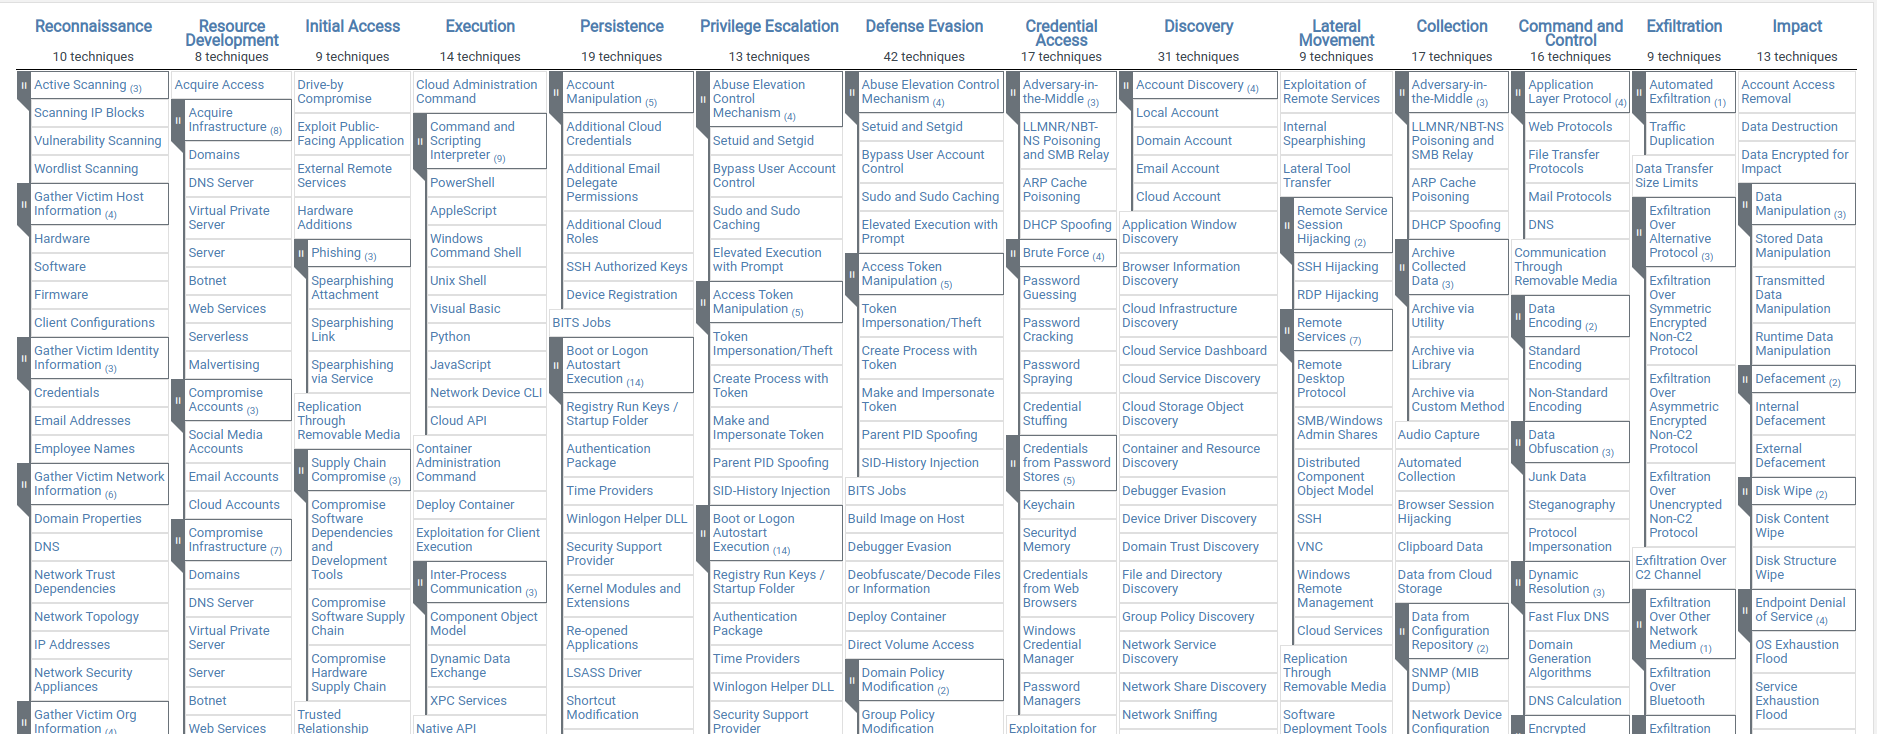
\includegraphics[width=\textwidth]{assets/mitre_attack_matrix.png}
    \caption{MITRE ATT\&CK Matrix for Enterprise}
    \label{fig:mitre_attack_matrix}
\end{figure}

Per identificare più precisamente le tipologie di malware che stiamo trattando, si va ad usare il \emph{MITRE ATT\&CK® Framework} (Adversarial Tactics, Techniques, and Common Knowledge)
\footnote{Pagina ufficiale MITRE ATT\&CK: \url{https://attack.mitre.org/}}.

Si tratta di una base di conoscenza sviluppata da MITRE Corporation, che include tattiche e adversary techniques, basata osservando gli avvenimenti nel mondo reale. Nato nel 2013 con lo scopo di descrivere le più comuni tattiche, tecniche e procedure \emph{(TTP)} usate nei sistemi Windows enterprise, ad uso interno MITRE, è poi diventato lo standard de-facto per la descrizione di tali aspetti di un attacco
\cite{mitre_attack_framework_introduction}, per far fronte all'assenza di una tassonomia comune per la descrizione dei TTP.

Si focalizza sulle interazioni che il malware ha col sistema target, e raggruppa questi comportamenti in tattiche per fornire più contesto sulla tecnica utilizzata.
\begin{itemize}
    \item Le \textbf{tattiche} sono il \emph{perché} di una tecnica, indicando l'obiettivo che si intende perseguire, e servono da contenitore per le varie tecniche; nello standard iniziano per \texttt{TA} (es: \texttt{TA0043} - Reconnaissance - Ricognizione, l'avversario va ad ottenere informazioni sul sistema per capire come muoversi)
    \item Le \textbf{tecniche} invece sono il \emph{come} di una specifica azione, e potrebbero far dedurre anche il \emph{cosa} un avversario ottiene come risultato della sua azione - particolarmente utile nella tattica TA0007 Discovery, dove si cerca di studiare la composizione del sistema target. \\
    Una tecnica è spesso composta da sotto-tecniche per essere ancora più specifici.
    Ad esempio, la tecnica \texttt{T1595.002} Vulnerability Scanning (dove si va capendo i software disponibili sul sistema target e la loro versione, con il possibile scopo di verificare se si allinea a una specifica versione vulnerabile di cui l'avversario già dispone di un exploit) è sotto-tecnica di \texttt{T1595} Active Scanning, e fa parte della tattica \texttt{TA0043} Reconnaissance vista al punto precedente.
\end{itemize}

Nella matrice in figura \ref{fig:mitre_attack_matrix}, le tattiche sono le colonne e le tecniche sono le celle, possibilmente composte da sotto-tecniche.

Viene usato anche per l'integrazione con la Cyber Threat Intelligence, che vedremo nella sezione \ref{chap:cyber_threat_intelligence}, punto focale anche degli strumenti realizzati nel progetto.

\section{Cyber Kill Chain}
Partendo dalle tattiche appena viste, possiamo costruire ciò che è noto col nome di \emph{Cyber Kill Chain}.
Si tratta di un modello simile al MITRE ATT\&CK framework (sez. \ref{chap:mitre_attack}), ma segue un diverso approccio. Qui infatti si vanno a ripercorrere le 7 tipiche fasi cronologiche di un attacco ad un sistema informatico, fornendo una panoramica più ad alto livello.

\begin{figure}[h]
    \centering
    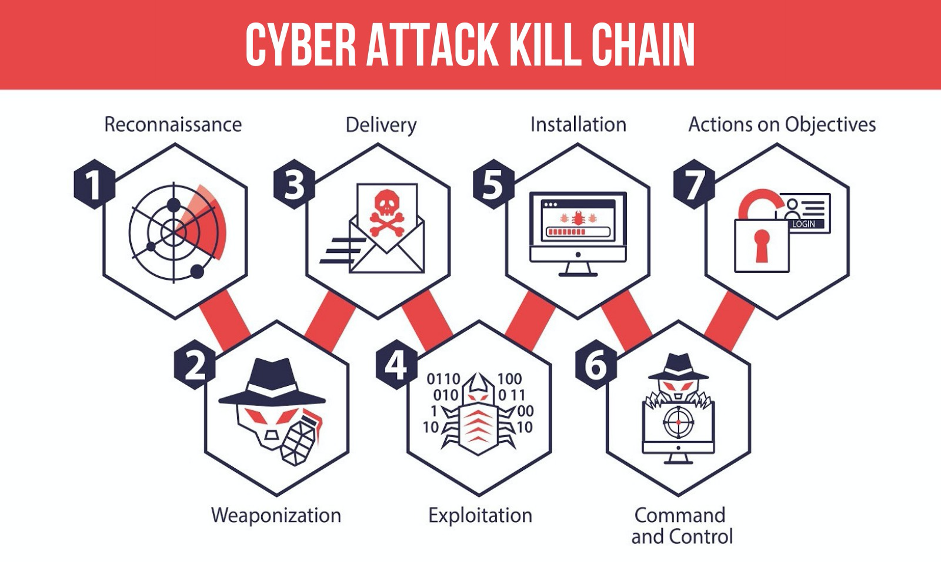
\includegraphics[width=0.6\textwidth]{assets/cyber_kill_chain.png}
    \caption{(crediti immagine: "Fondazione F3RM1")}
    \label{fig:cyber_kill_chain}
\end{figure}

Si compone delle seguenti fasi \cite{cyber_kill_chain_360}, portando un esempio tipico:
\begin{enumerate}
    \item \textbf{Ricognizione}: identificazione dei punti di accesso a un sistema e sue vulnerabilità, derivabili tramite analisi attiva (uso di strumenti come \emph{nmap} in maniera più o meno aggressiva) o passiva, leggendo informazioni già da fonti note (come \emph{Shodan.io} partendo da un indirizzo IP): ad esempio, possiamo notare come siano presenti ed esposti servizi con versioni obsolete / vulnerabili
    
    \item \textbf{Armamento}: creazione del vero e proprio malware da utilizzare nell'attacco, nell'intento di sfruttare la vulnerabilità individuata - ad esempio creiamo un pacchetto IP con scapy

    \item \textbf{Consegna}: il payload creato deve essere consegnato alla vittima in qualche modo, come una mail di phishing o un form di una pagina del sito web - quindi inviamo il pacchetto al server al suo indirizzo IP pubblico

    \item \textbf{Exploit}: nella realtà dei fatti, si sta sfruttando una vulnerabilità individuata - nel nostro caso reale, potremmo aver scatenato una RCE (Remote Code Execution) o altre tecniche

    \item \textbf{Installazione}: dopo la riuscita dell'exploit, si scarica e avvia il payload malevolo, cercando di bypassare strategie esistenti di rilevazione, usando metodologie come obfuscation - nell'esempio, possiamo installare una reverse shell ad avvio automatico in file come `~/.bashrc` o `~/.profile`

    \item \textbf{Command and Control (C\&C)}: andiamo a instaurare un canale di comunicazione tra noi e la vittima, così da controllarlo da remoto - qui possono essere utili strumenti come Havoc C2.

    \item \textbf{Azioni sugli obiettivi}: eseguiamo le azioni più disparate, in base a ciò che vogliamo fare noi come attaccanti, come leggere un file contenenti informazioni sensibili o eseguire il dump del database
\end{enumerate}

\section{Sistemi di protezione}
Ora che abbiamo visto tutte queste minacce, viene spontaneo chiedersi come sia possibile proteggersi.

L'\textbf{antivirus} e' lo strumento base per la protezione dei singoli computer. Gli antivirus tipicamente ricercano i malware noti (utilizzando database di firme) analizzando i file memorizzati su disco. Il limite dell'approccio basato su firme (o signature dei malware) è quello di scovare solamente i malware noti. 

Ben più potente è l'EDR, acronimo di \textbf{Endpoint Detection and Response}, che sfrutta l'\emph{analisi comportamentale} per rilevare e contrastare anche minacce sconosciute, basandosi sui loro comportamenti. Ad esempio, se vediamo che, dopo aver aperto un file scaricato da Internet, il processo del programma che ne permette la visualizzazione inizia a fare operazioni fuori dal normale funzionamento, come aprire una shell o modificare file o registri di sistema, sicuramente andrà terminato e riportato come incidente, che poi andrà gestito da chi di competenza.
La sostanziale differenza è il passaggio da semplice analisi su disco a una profonda analisi comportamentale, sfruttando strumenti forniti dal sistema operativo come Microsoft ETW \emph{(Event Tracing for Windows)} o eseguire l'hooking delle syscall manualmente - tecnica ben più complessa ed error-prone.

Infine, con un XDR (\textbf{eXtended Detection and Response}) andiamo ad allargare gli elementi sotto la protezione del software in questione, permettendo un'integrazione anche con reti, firewall, log di sicurezza e molto altro.
In questo modo, ha la potenza di aggregare e correlare eventi da più fonti, rilevando minacce sofisticate che verrebbero altrimenti ignorate.
Un esempio in questa categoria è \emph{SentinelOne XDR}.

\section{Cyber Threat Intelligence}
\label{chap:cyber_threat_intelligence}
L'area di Threat Intelligence si occupa di raccogliere tutta una serie di dati dai vari elementi,
per poi aggregarli e compiere analisi sulle informazioni ottenute, al fine di rilevare minacce anche sofisticate e prendere decisioni sulla sicurezza in maniera più veloce e consapevole.

La Threat Intelligence è un tassello estremamente importante nella sicurezza di un sistema informatico, soprattutto se unito al MITRE ATT\&CK framework: documentando i profili con cui l'avversario opera (come \texttt{APT29} - i profili sono insiemi di attività tipiche del modo di operare di alcuni gruppi nel panorama cyber), ma anche individuando la tecnica più efficacemente così da raggruppare tra loro più attacchi con caratteristiche comuni.
In questo modo, è possibile focalizzarsi maggiormente sulle tecniche che sono maggiormente usate in un dato profilo di attacco.

Esempi di come particolari avversari, delineati sotto un profilo, usano le proprie tecniche sono documentati nella pagina ATT\&CK corrispondente.
Studiandone la metodologia di attacco, è possibile replicarlo in fase di emulazione \emph{(Adversary Emulation)} per capire fino in fondo come difendersi da attacchi similari, e testare le proprie difese, nonché eseguire test di rilevazione.

Per questo e altri motivi, come vedremo, nella prima fase di analisi integreremo questo framework per la categorizzazione delle capabilities di un eseguibile.

\medskip

Un altro importante ruolo della Threat Intelligence, maggiormente vicino al progetto realizzato, è quello di analizzare i malware coinvolti negli attacchi noti o forniti da clienti qualora ne chiedessero l'analisi approfondita. Proprio a questo scopo, il proprio lavoro viene nettamente agevolato da strumenti di analisi automatica più estendibili possibile, così da avere fin da subito tutti i dati su cui lavorare.

\section{Contesto d'uso del progetto}
Una volta vista una panoramica di questo ambito della sicurezza informatica,
andiamo ad analizzare il contesto in cui si va ad inserire il progetto realizzato.

L'azienda ospitante offre, come suo core business, sistemi di EDR e XDR.
Questi sistemi usano programmi Agent installati nei vari endpoint, che sonde usate per analizzare il traffico di rete nei vari livelli ISO-OSI, nonché analisi sui dispositivi OT.

Soprattutto in riferimento all'Agent installato sugli endpoint, esso andrà a rilevare eseguibili con comportamenti anomali o sconosciuti e li andrà ad inviare al sistema di Threat Intelligence, che valuterà con una data confidence se siano o meno malevoli.
La capacità di eseguire detection di alta qualità è uno dei tratti distintivi tra le diverse soluzioni di sicurezza esistenti sul mercato e ha una diretta ripercussione sulla soddisfazione del cliente finale dell'azienda, oltre alla propria reputazione come brand.
Proprio in questo punto cruciale, viene l'esigenza dietro il progetto realizzato.

\subsection{Il problema da risolvere}
Lo scopo principale è la costruzione di un sistema proprietario per l'analisi automatizzata di malware, eliminando le ultime dipendenze con servizi terzi quali VirusTotal, sia per un fattore economico che di flessibilità nei propri prodotti.

Un aspetto importante mantenuto chiaro per tutto il corso del progetto è proprio la flessibilità che deve essere garantita a questo nuovo strumento di essere esteso e maggiormente integrato nel corso della propria esistenza. Com'è intuibile infatti, il sistema qui creato verrà successivamente usato come base per la propria architettura di analisi malware automatizzata, che si andrà ad interfacciare con i vari prodotti.

\subsection{Interfacciamento con gli altri servizi}
\label{chap:intro_interface_with_other_services}

Il progetto si andrà ad integrare nella nuova architettura di sistema proprietaria dell'azienda ospitante.
Seppur è ancora in costruzione, per cui alcuni aspetti potrebbero variare tra il momento della scrittura e la loro effettiva realizzazione, ne viene delineato lo stato dell'arte.

Il punto di partenza è rappresentato dall'Agent, nominato poco fa e installato sui vari endpoint ove possibile, che raccoglie eseguibili sospetti e che reputa necessitino un'analisi più approfondita.
Siccome spesso si trova all'interno di una rete isolata, dove non è permessa la comunicazione con qualsiasi host Internet, può inviare gli eseguibili al COS. Più precisamente, inizialmente l'Agent non conosce ancora se siano già presenti analisi, così per questioni di efficienza invia solo il suo hash, inviando poi l'intero file solo in caso di esito negativo.

Il COS si occuperà di mantenere una coda di analisi, per non sovraccaricare il resto dei sistemi.
Invierà il file o l'hash ad FSL, che si pone come middleware per le API della Threat Intelligence.

Attualmente viene interrogata l'API di VirusTotal Enterprise per ottenere il maggior numero di informazioni, ma come abbiamo detto questa è la parte più critica a causa degli ingenti costi (fig. \ref{fig:fsl_general_arch_vt_success}).

In caso negativo, verrà invocato il progetto qui realizzato. Quindi, l'Agent invierà il file (non più l'hash) al COS, che lo inoltrerà alla nostra Sandbox, che si compone di una parte di analisi statica e di una dinamica (fig. \ref{fig:fsl_general_arch_sandbox_invoke}). Come vedremo, la fase di analisi statica avrà come trigger l'upload di un file su uno specifico bucket S3.

\section{Architettura generale della Sandbox}

Il sistema di analisi qui realizzato, chiamato per brevità anche \emph{Sandbox},
si compone di due parti, indipendenti l'una dall'altra al fine di mantenere una massima modularità.
Qui sono riportate come introduzione le due architetture in linea di massima, che verranno poi ben dettagliate nelle apposite sezioni di seguito.

Per quanto concerne l'aspetto statico, ci si avvarrà di Amazon Web Services per il funzionamento,
sfruttando principalmente i servizi di cloud storage S3 Bucket e di esecuzione Lambda, per minimizzare i costi e avere un sistema flessibile.
Una volta analizzato il file, la Threat Intelligence, mediante le sue API, riceverà gli stati di inizio e fine del processo, inclusi i risultati in un formato JSON concordato. Lo andrà a salvare e lo userà nelle future richieste con lo stesso hash (fig. \ref{fig:fsl_general_arch_sandbox_cached}).

Al contempo, l'aspetto dinamico si avvale di una già nota sandbox open-source quale Cuckoo Sandbox,
su cui è stato costruito il resto del sistema completo,
andando a installare il software, configurare il sistema a livello di firewall e SystemD Unit,
nonché creare nuovi moduli al fine di integrare tool nuovi, e un sistema di reporting che si basa su un client Python sviluppato appositamente per lo scopo.

\begin{figure}
    \centering
    \begin{subfigure}[b]{0.48\textwidth}
        \centering
        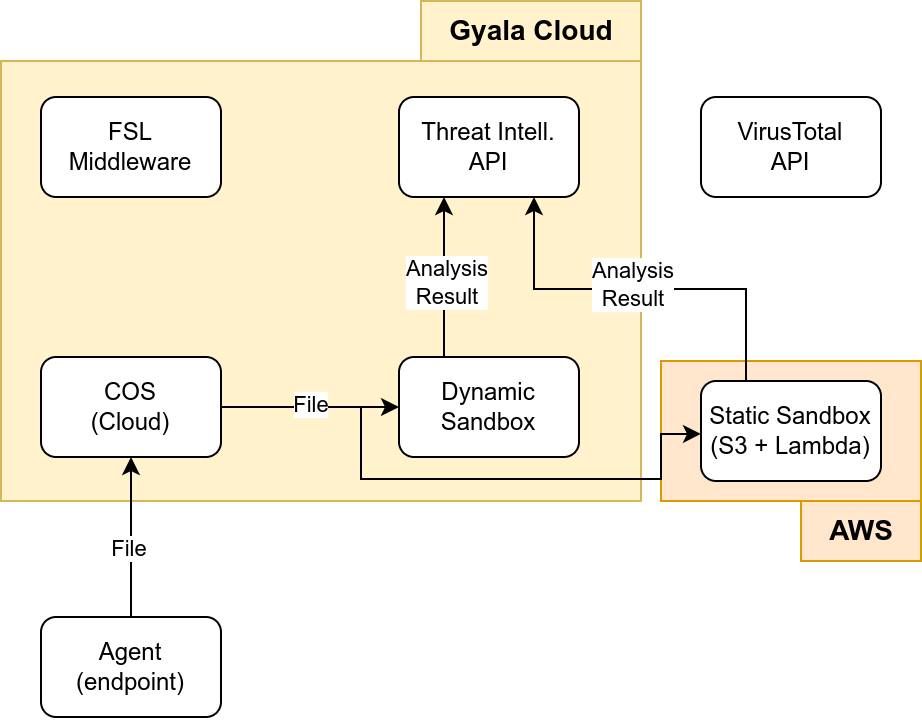
\includegraphics[width=\textwidth]{assets/fsl_general_arch_sandbox_invoke.png}
        \caption{Necessario invocare la sandbox}
        \label{fig:fsl_general_arch_sandbox_invoke}
    \end{subfigure}
    \begin{subfigure}[b]{0.48\textwidth}
        \centering
        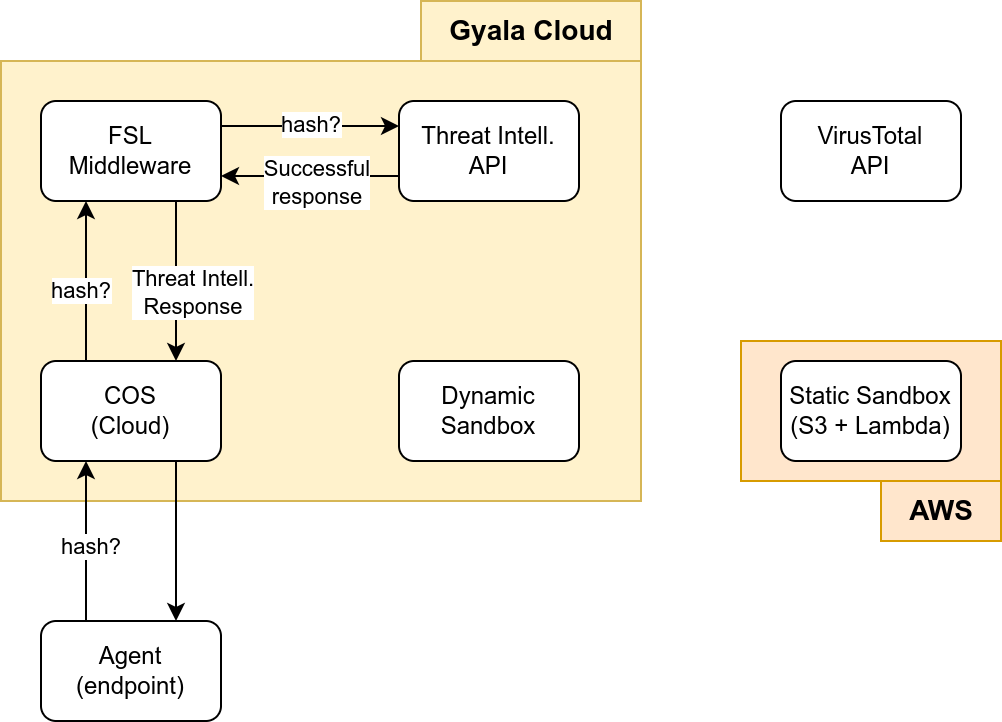
\includegraphics[width=\textwidth]{assets/fsl_general_arch_sandbox_cached.png}
        \caption{Risultati della Sandbox già in database}
        \label{fig:fsl_general_arch_sandbox_cached}
    \end{subfigure}
    \hfill
    \vspace{0.5cm}
    \hfill
    \begin{subfigure}[b]{0.48\textwidth}
        \centering
        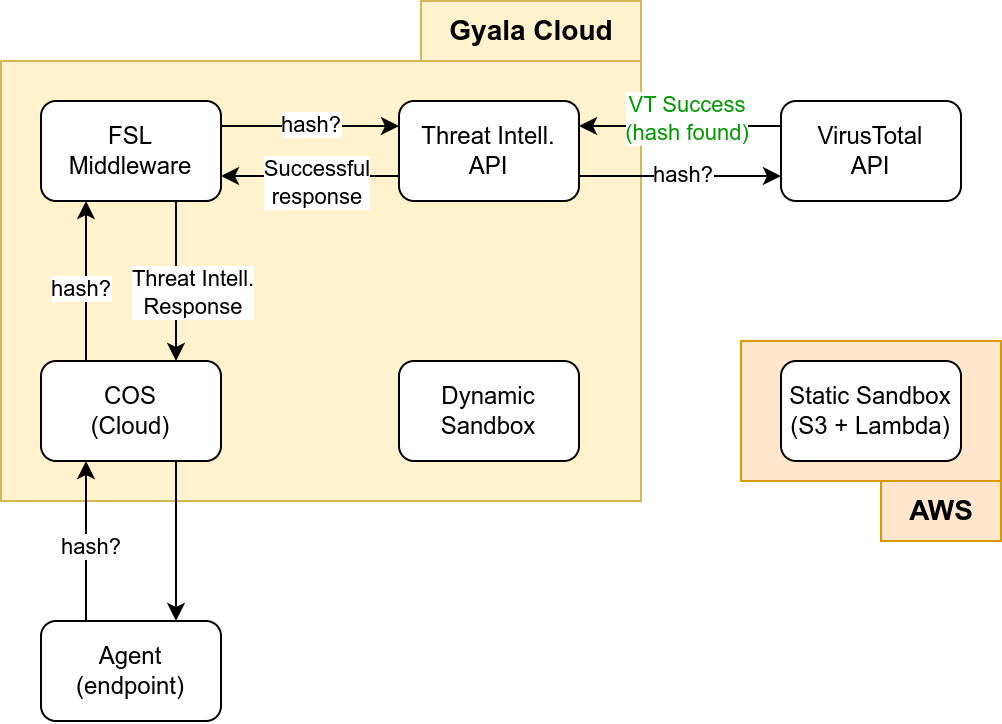
\includegraphics[width=\textwidth]{assets/fsl_general_arch_vt_success.png}
        \caption{Vecchio flusso prima della creazione della Sandbox}
        \label{fig:fsl_general_arch_vt_success}
    \end{subfigure}
    \caption{Schema generale di funzionamento dell'architettura nei vari casi}
    \label{fig:fsl_general_arch}
\end{figure}
\chapter{Analisi statica}
Il primo passo di questo processo di analisi riguarda in primo luogo un approccio di tipo statico.

Questo tipo di analisi è usato per fare una prima esaminazione senza eseguirli su un sistema.
Per arrivare a tali risultati, si ispeziona il codice del file del malware, alla ricerca di varie caratteristiche, in base a quale strumento stiamo usando e al suo scopo.
Possiamo andare alla ricerca, più o meno approfondita, di chiamate di sistema particolari, indizi di offuscamento o crittografia anche tramite un'analisi dell'entropia di alcune sezioni del file, nonché più direttamente degli IoC già noti.
Si possono usare numerose tecniche, tra cui:

\begin{itemize}
    \item \textbf{Disassemblaggio o decompilazione} al fine di andare ad esaminare il codice più o meno ad alto livello del sorgente originale dell'eseguibile, anche se spesso questa pratica resta difficoltosa per tutte le ragioni dietro la reverse-engineering, con particolare attenzione degli autori del malware di rendere tecniche come questa il più difficili possibile
    \item \textbf{Analisi delle stringhe} per identificare IoC particolari come URL noti, indirizzi IP, o anche semplicemente nomi di chiavi di registro o file che normalmente non dovrebbe andare a toccare in un normale funzionamento
    \item \textbf{Estrazione dei payload} integrati all'interno del file, come exploit nascosti / crittografati o anche lo stesso codice del vero eseguibile, come nel caso dei file pacchettizzati, che tratteremo nelle successive sezioni
\end{itemize}

Infine, non necessariamente si deve trattare di un eseguibile: può anche essere analizzato un documento Office o un file PDF, anch'essi noti per essere potenziali vettori di attacco, includendo delle macro o del codice eseguibile al proprio interno.

\section{Struttura binari}
\label{chap:static_analysis_binary_structure}
Prima di andare nel dettaglio di quali tecniche sono state adottate per avere un sistema di analisi statica quanto più completo possibile, bisogna andare a illustrare sommariamente la struttura di un file binario.

Innanzitutto, un file eseguibile contiene sia codice che dati, ed è diviso in \textbf{sezioni}, che possono avere diversi permessi di lettura (read-only) o scrittura (read-write).
Questo è un dettaglio più importante di quanto ci aspetteremmo perché ad esempio un eseguibile potrebbe compiere tecniche di modifica della propria sezione di codice, impostandola come read-write, potendo eludere così in maniera piuttosto significativa tecniche di analisi statica, poiché il vero codice del software sarà creato durante la sua stessa esecuzione, e nella fase statica (come dice il nome stesso) non andiamo a lanciare alcun programma.

Un'altra area comune e rilevante è la \textbf{symbol table}, o "tabella dei simboli".
Questa contiene riferimenti a funzioni o variabili poste in altri file o librerie esterne, che nella prima fase di \emph{Assembling} sono stati trasformati in degli \emph{object file} distinti,
e come tali sono rilocabili, ossia non dipendono già da particolari indirizzi in memoria.
Quindi contengono riferimenti simbolici ad altri componenti, di cui avranno bisogno nella fase di Linking.

Proprio successivamente al Linking, abbiamo un singolo file binario, e questo avrà una tabella dei simboli più ridotta, ma pur sempre contenente riferimenti a funzioni contenute in librerie di sistema (si parla di librerie linkate dinamicamente).
Un attaccante potrebbe aumentare il più possibile il numero di librerie linkate staticamente, così da nasconderne il proprio utilizzo.
Un'altra tecnica molto usata in vari contesti è lo \emph{stripping}, eliminando dalla symbol table tutti i riferimenti alle funzioni esportate nel file stesso. Possiamo vedere un esempio di questo fenomeno nel caso dei file ELF su Linux in figura \ref{fig:elf_symtab}.

Di seguito, vediamo le principali peculiarità a seconda del sistema operativo a cui si riferiamo.

\subsection{ELF}
Il formato ELF \emph{(Executable and Linkable Format)} è proprio dei sistemi Linux, ma non solo, infatti è usato anche in vari microcontrollori, o console da gioco come la Nintendo Wii e la PlayStation \cite{forensic_friday_execs}.
Viene usato per file eseguibili, o anche file object comunemente indicati con l'estensione \texttt{.o}, shared libraries aventi estensione \texttt{.so} o core dumps.

Si compone di un header, descritto completamente nel file \texttt{sys/elf.h} e visibile in dettaglio in figura \ref{fig:elf_header}, contenente varie informazioni tra cui le più importanti come il tipo di file (\texttt{e\_type}), se eseguibile o uno tra quelli citati in precedenza,
il magic number con cui possiamo riconoscere che si tratta di un ELF,
l'architettura per la quale è stato compilato (\texttt{e\_machine})
e l'indirizzo di memoria virtuale, indicato come un offset all'interno del file, che il sistema operativo dovrà eseguire per lasciare il controllo al nuovo processo nato (\texttt{e\_entry}).

\begin{figure}[!ht]
    \centering
    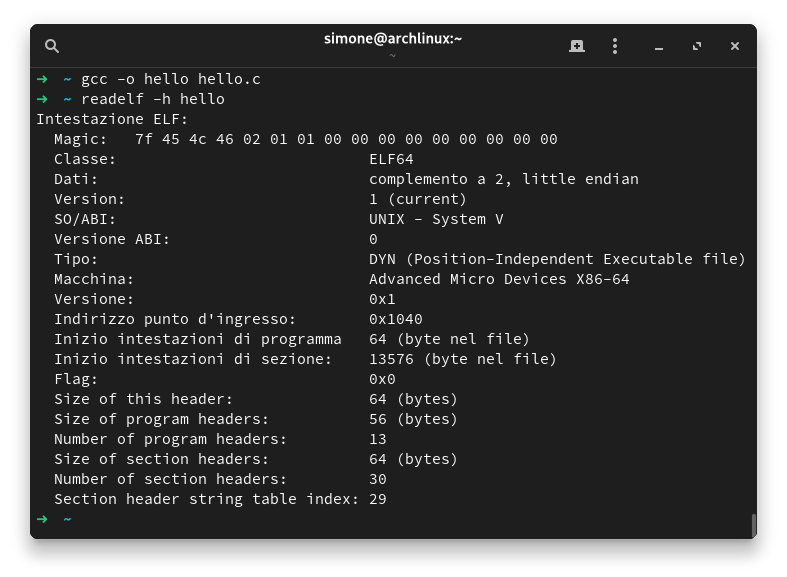
\includegraphics[width=0.6\textwidth]{assets/elf_header.png}
    \caption{Header di un file ELF, letto con readelf}
    \label{fig:elf_header}
\end{figure}

Ma al suo interno troviamo anche le sezioni, tra cui le più rilevanti, con le possibili misure di sicurezza che se mancano potrebbero essere un indicatore che dovrebbe essere portato all'attenzione: \cite{forensic_friday_execs}
\begin{itemize}
    \item \texttt{.text} contiene il codice principale del programma, e rappresenta il focus principale di ogni analisi sul file binario; ha il tipo \texttt{SHT\_PROGBITS} affinché sia eseguibile ma non scrivibile, protezione assolutamente voluta in un programma standard
    \item \texttt{.data} e \texttt{.rodata} contengono i dati del programma, come le variabili o le costanti, a seconda che sia una sezione scrivibile o meno - ad esempio, rilevare un valore di entropia molto alta in questa sezione può essere indice di uso di compressione o crittografia, e va valutato caso per caso se è un comportamento che ci aspettavamo o può essere indicatore di qualcosa di malevolo, proprio per la sua volontà di rendere sempre più difficile l'analisi senza una esecuzione del programma stesso
    \item \texttt{.init} e \texttt{.fini} contengono le procedure di inizializzazione e finalizzazione da eseguire prima del main o prima della terminazione del processo a seguito della fine del normale flusso di esecuzione
\end{itemize}

\begin{figure}[!htb]
    \centering
    \begin{subfigure}[t]{0.48\textwidth}
        \centering
        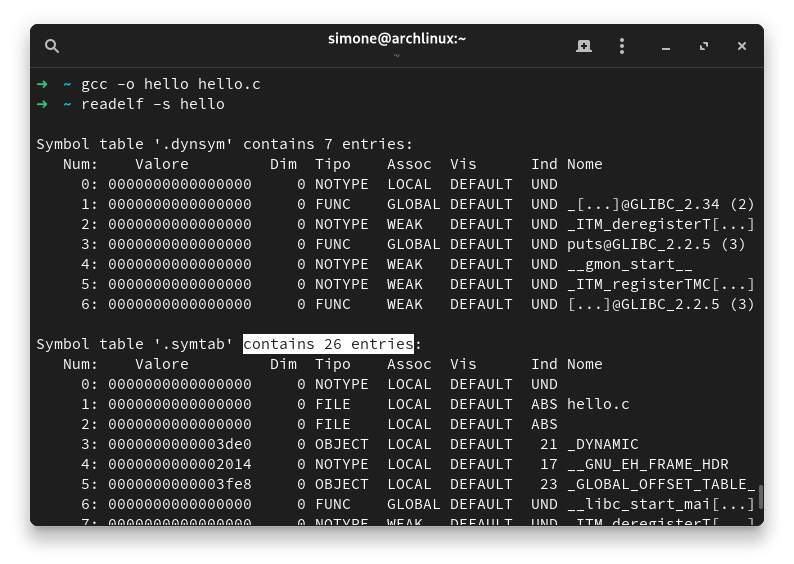
\includegraphics[width=\textwidth]{assets/elf_symtab_full.png}
        \caption{Symbol table originale}
    \end{subfigure}
    \begin{subfigure}[t]{0.48\textwidth}
        \centering
        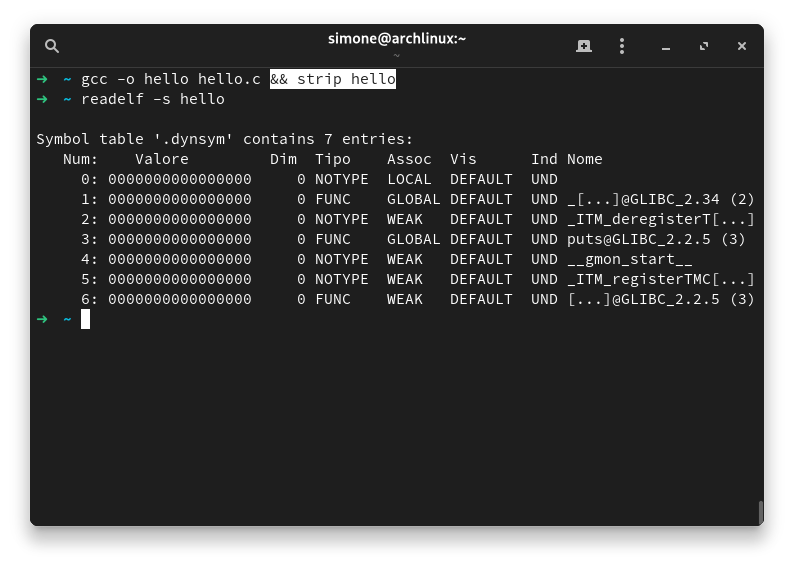
\includegraphics[width=\textwidth]{assets/elf_symtab_stripped.png}
        \caption{Symbol table dopo strip}
    \end{subfigure}
    \caption{Confronto delle symbol table prima e dopo lo strip}
    \label{fig:elf_symtab}
\end{figure}


\subsection{PE}
PE sta per \textbf{Portable Executable} ed è il formato usato nei sistemi Microsoft, derivato dal formato \emph{COFF} di Unix, motivo per cui è spesso identificato come PE/COFF. \cite{forensic_friday_execs}

Viene usato per vari tipi di file, tra cui eseguibili, DLL (Dynamic Link Libraries) e object file.

Anch'esso ha il proprio magic number ai fini di essere identificato correttamente, ed è composto da più header, dove possiamo notare tutta la sua evoluzione come formato. Inizialmente troviamo header specifici di MS-DOS, e successivamente header più caratteristici delle nuove versioni dei PE, includendo sia informazioni di base comuni agli ELF, come il numero di sezioni, di simboli e l'architettura, ma anche la firma digitale dell'immagine del programma per proteggersi da tampering e verificare che l'eseguibile sia realmente proveniente dalla corretta azienda, a meno di leak delle chiavi privati usate per la firma stessa.
\footnote{Maggiori dettagli sono disponibili alla pagina \url{https://learn.microsoft.com/en-us/windows/win32/debug/pe-format}}

\section{Capa: capabilities}
\label{chap:capa}
Per i test che vedremo in questa sezione, sono stati scaricati \textbf{40 sample} di malware reali da VirusTotal casualmente, e nelle varie fasi di miglioramento ed evoluzione, soprattutto in merito all'analisi delle capabilities, sono stati fatte numerose prove usando come campioni proprio questi sample.

Per \emph{capabilities} intendiamo le funzionalità che va a usare il programma, ossia ciò che è capace di svolgere durante la propria esecuzione. Esempi di capabilities possono essere la connessione a un server remoto, la modifica di chiavi di registro, o la creazione di un processo figlio, solo per citarne qualcuna.

\begin{figure}[!htb]
    \centering
    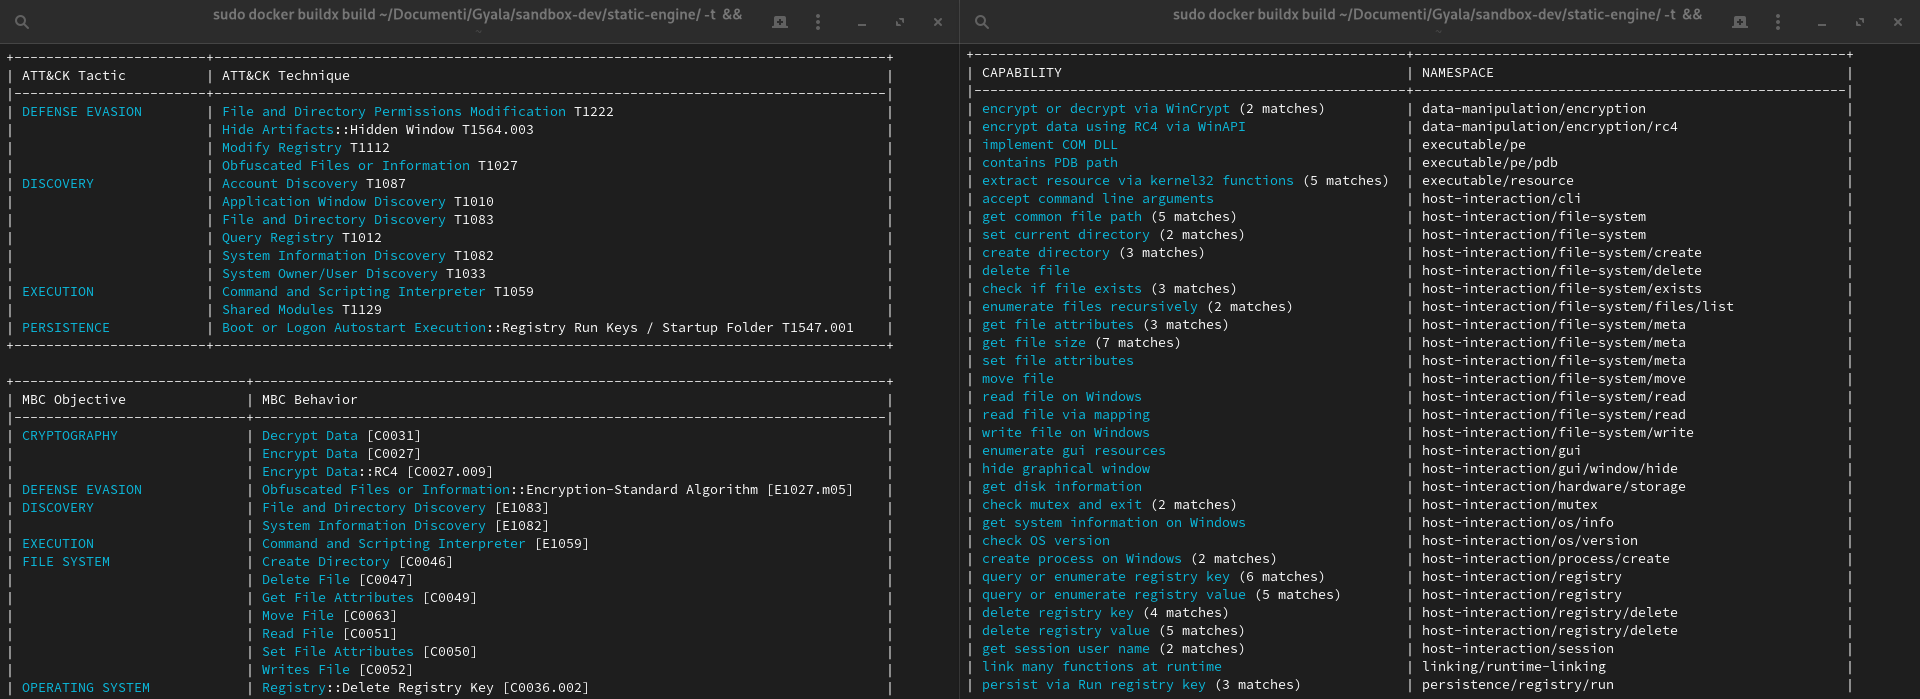
\includegraphics[width=\textwidth]{assets/capa_example_invocation.png}
    \caption{Esempio di esecuzione di capa su pafish64}
    \label{fig:capa_example_invocation}
\end{figure}

Questa estrazione infatti sfrutta lo strumento \textbf{capa},
\footnote{\url{https://github.com/mandiant/capa}}
visto in figura \ref{fig:capa_example_invocation},
tool open-source creato da Mandiant, una delle aziende leader del settore e ora parte di Google,
che permette di andare ad individuare delle capabilities all'interno di un file eseguibile
sfruttando delle regole aventi un proprio formato.
Funziona andando prima ad estrarre delle \emph{features} come le stringhe incluse, codice disassemblato, control flow o file importati.
Poi vengono lanciate le regole su queste features al fine di trarne un'implicazione logica e ottenere informazioni valide a fronte di un match con una o più regole capa.

Si è rilevata la \emph{scelta ottimale} per il progetto per la sua natura open-source, per la grande azienda che è dietro la sua realizzazione, ma soprattutto per la potenza espressiva delle sue regole.
Possiamo scrivere regole in un file di testo in formato YAML, seguendo la semplice struttura richiesta da capa, per aggiungere in futuro ulteriori regole, sia internamente che estratte da altri contributori nei propri repository. Infine, è possibile anche organizzarli per tag, così decidendo volta per volta quali specifiche regole eseguire, garantendo massima flessibilità.

Il processo di feature extraction si basa in gran parte sull'header che abbiamo appena menzionato nella sezione \ref{chap:static_analysis_binary_structure}, comprese informazioni sulle funzioni esportate, tabella dei simboli (SymTab) e sezioni. Inoltre, il processo di disassemblaggio è molto complesso perché punta sia ad individuare features quali API calls, istruzioni speciali o riferimenti di stringhe/numeri poste in altre sezioni dell'eseguibile (come \texttt{.rodata} per le costanti), ma anche a ricostruire il control-flow minimizzando falsi positivi in caso di dead code o per distinguere tra funzioni e altri \emph{scope}. Alla base di questo step, c'è \texttt{ViviSect Feature Extractor}. \cite{capa_mandiant_blogpost}

Una volta ottenute tutte le features di interesse, si procede a fare il match con le regole.
Una regola capa è una combinazione logica strutturata di match di varie features più di basso livello, per giungere alla conclusione di presenza o assenza di una determinata capability all'interno del software in analisi, espresse sotto forma di file \texttt{YAML}.

Nelle regole, può venir inoltre specificata la tecnica e quindi la tattica, secondo il MITRE ATT\&CK Framework (sez. \ref{chap:mitre_attack}), come visibile nell'output del comando (fig. \ref{fig:capa_example_invocation}).
Questa rappresenta un grande vantaggio per l'integrazione con altri strumenti di Threat Intelligence, per le stesse ragioni favorevoli dell'adozione del framework.

\begin{figure}[!htb]
    \centering
    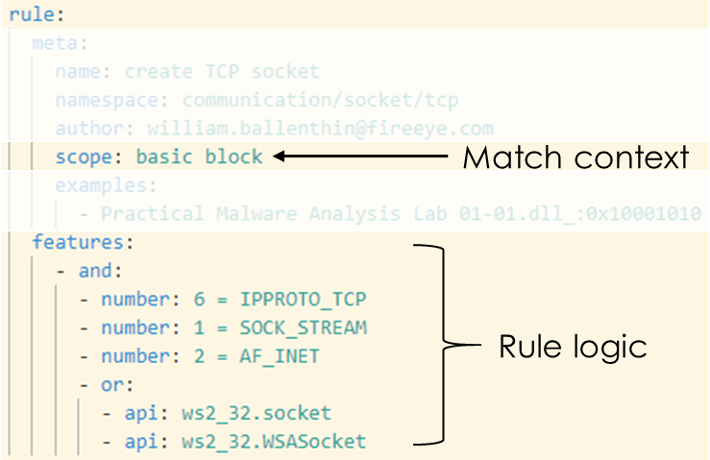
\includegraphics[width=0.6\textwidth]{assets/capa_example_rule.png}
    \caption{Regola capa per rilevare la creazione di un socket TCP}
    \label{fig:capa_rule_socket_tcp}
\end{figure}

Tuttavia, non tutti gli eseguibili sono supportati da capa, proprio per i motivi precedentemente elencati riguardanti i file offuscati o pacchettizzati. A questo scopo, sono presenti all'interno del set standard di capa, delle regole
(sotto il namespace \texttt{internal/limitation/file} \footnote{\url{https://github.com/mandiant/capa-rules/tree/master/internal/limitation/file}})
che se hanno un match col file in analisi, capa si arresterà non ritenendo più affidabili i propri risultati.
Questo, come vedremo nel prossimo paragrafo, ci costerà troppo tempo e andrà risolto in un altro modo, individuato in \ref{chap:static_custom_file_detector}.

\subsection{Analisi dell'uso delle risorse}
Vogliamo analizzare l'uso di risorse da parte di capa con una varietà di file diversi, ossia i 40 sample precedentemente citati da VirusTotal, in termini di spazio e tempo, provando a cercare delle correlazioni con altri dati a nostra disposizione, al fine di eventualmente poter eseguire delle ottimizzazioni.

Bisogna ricordare infatti che il ben più ampio sistema con cui questo progetto si andrà in futuro a interfacciare lavora diverse migliaia di sample ogni mese, per cui è fondamentale ridurre gli sprechi.

All'interno di una macchina virtuale, è stato installato il tool \texttt{capa} insieme ai sample da mettere sotto esame.
Prima di fare ogni tipo di studio, abbiamo bisogno di estrarre dei dati, ottenibili con uno script Python che legge lo stderr del comando, nonché il suo tempo di esecuzione.

Uno dei dati più significativi è il numero di funzioni o blocchi che devono essere analizzate dal feature extractor.
Usando matplotlib, andiamo a validare questa supposizione o confutarla, visualizzando i due elementi in un grafico (fig. \ref{fig:capa_correlation_plot}).

\begin{figure}[!htb]
    \centering
    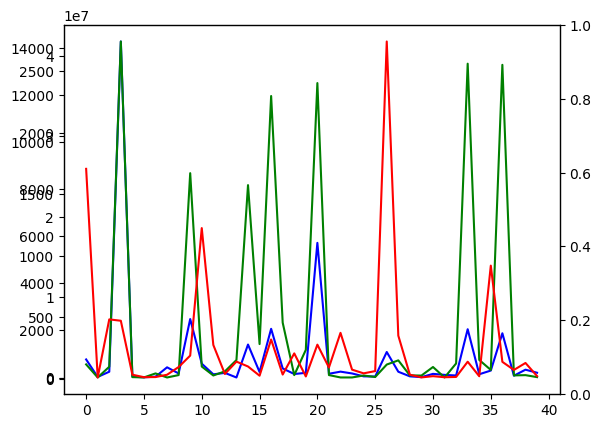
\includegraphics[width=0.6\textwidth]{assets/capa_correlation_plot.png}
    \caption{Correlazione tra tempo di esecuzione (blu) e numero di funzioni/blocchi (verde), assenza di relazione con la dimensione del file (rosso)}
    \label{fig:capa_correlation_plot}
\end{figure}

Siccome su questa metrica non possiamo intervenire in alcun modo, focalizziamoci sull'evitare l'esecuzione di analisi su file che non sono supportati.

%%%%%%%%%%%%%%%%%%%%%%%%%%%%%%%%%%%%%%%%%%%%%%%%%%%%%%%%%%%%%%%%%%%%%%%%%%%%%%%

\subsection{File offuscati}
\label{chap:static_analysis_obfuscated}
Per prima cosa è stato notato come il tool restituisse un diverso \emph{exit code} in base alla corretta esecuzione della feature extraction o meno (listing \ref{code:capa_exit_code}). Da ciò, possiamo rilevare quando un file poteva essere scartato a monte o l'esecuzione di capa ha portato a risultati utili per cui le risorse sono state ben spese.

\begin{code}
\caption{Distinzione tra gli exit code di capa}
\begin{minted}{bash}
function test_file_with_capa() {
    capa "$1" 2>&1 | grep "WARNING:capa: Identified via"
    echo "Exit code (capa): ${PIPESTATUS[0]}"
}

$ test_file_with_capa ./executables/visual_basic_file.exe
WARNING:capa: Identified via rule: (internal) Visual Basic file limitation
Exit code (capa): 14

$ test_file_with_capa ./executables/standard_pe.exe
Exit code (capa): 0
\end{minted}
\label{code:capa_exit_code}
\end{code}

Da qui, abbiamo potuto categorizzare i vari sample in gruppi sulla base del tipo di file, che sia standard (\texttt{pe}) o non supportato da capa (\texttt{packed}, \texttt{installer}, ...).
Creiamo quindi uno script Python che sia in grado di automatizzare questa azione, sia sulla base dell'exit code che dell'output sullo stderr. Otteniamo un JSON come il seguente (estratto per sintesi):

\begin{minted}[samepage]{json}
{
  "./b9c32debb4.exe": "installer",
  "./9f79ea539a.exe": "pe",
  "./4726c42b25.exe": "visualbasic",
  "./e49c42d0b1.exe": "pe",
  .....
}
\end{minted}

La distribuzione della tipologia dei file è riassumibile più graficamente nella figura \ref{fig:capa_file_type_split}, dove notiamo come circa la metà dei sample è difficilmente analizzabile con capa per difetti congeniti dell'analisi statica.
Siccome non possiamo agire direttamente su questo aspetto per eseguire il tool, il prossimo passo sta nel quantificare lo spreco di risorse che si verifica analizzando le capabilities di file che poi porteranno a un fallimento del processo, e se può essere conveniente a livello di trade-off costruire una soluzione per salvaguardare l'uso di risorse saltando del tutto la sua esecuzione (codice \ref{code:static_analysis_capa_count_wasted_time}).

\begin{figure}[!htb]
    \centering
    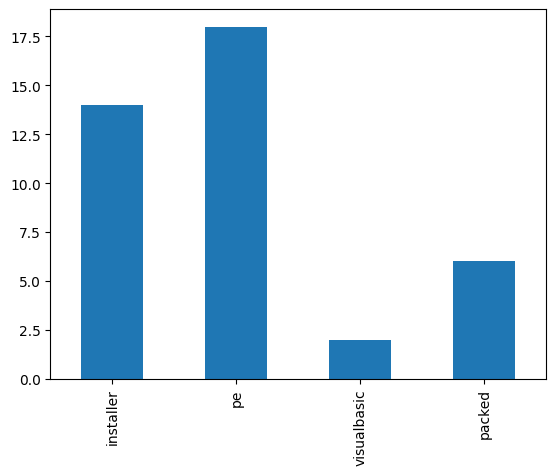
\includegraphics[height=1.8in]{assets/capa_file_type_split.png}
    \caption{Divisione dei sample per tipologia}
    \label{fig:capa_file_type_split}
\end{figure}

\begin{code}
\caption{Calcolo del tempo sprecato eseguendo capa su file non supportati}
\begin{minted}{python}
times = {
    k: v['elapsed_time']
    for k, v in times.items() if file_types[k] != 'pe'
}
avg_wasted_time = sum(times.values()) / len(times)
print(f'{avg_wasted_time:.2f} sec. per unsupported file (avg)')
# 58.77 sec. per unsupported file (avg)
\end{minted}
\label{code:static_analysis_capa_count_wasted_time}
\end{code}

Notiamo che ci mette \textbf{un'eccessiva quantità di tempo} per
eseguire il match delle regole le quali indicano a capa l'impossibilità a proseguire con una soddisfacente confidence, con una media di quasi \emph{un minuto per file}, che moltiplicato su tanti file diventa una grande quantità di tempo totale che potrebbe essere usato in maniera migliore.

\medskip

Ci basta avere i dati di ciò che stiamo trattando, ad esempio l'output desiderato in questo caso sarà del tipo:
\begin{minted}[samepage]{json}
{
    "capa": {
        "format": "packed",
        "arch": "i386",
        "os": "windows"
    }
}
\end{minted}

Come soluzione, dobbiamo trovare un sistema per riconoscere preventivamente che si tratti di un file che non è possibile analizzare con capa.

\subsection{Scrittura del parser}
Capa, al contrario di ciò che vedremo di seguito, è un tool da usare da CLI e offre un output testuale, come in figura \ref{fig:capa_example_invocation}.

Siccome al nostro strumento serve un output più machine-readable da restituire come risultato del processo di analisi, è stato scritto in Python un \textbf{parser} in grado di trasformare quel testo in un JSON.
Le chiavi principali sono come le 3 tabelle, ossia \texttt{capabilities}, \texttt{tactics} e \texttt{objectives}, oltre alla prima parte di \texttt{info} presente all'inizio, seguendo la struttura già fornita dall'output testuale.

Analizziamo com'è stato eseguito il parsing a un livello più astratto.
Prima di tutto, notiamo dalla figura \ref{fig:capa_example_invocation} come le linee vuote dividano le sezioni, quindi possiamo sfruttare questo fatto per stabilire la fine dell'una e il conseguente inizio dell'altra.
Poi, le linee che ci interessano iniziano per \texttt{|}, escluso l'inizio per \texttt{|---}. Così facendo arriviamo a un output similare a quanto in figura \ref{fig:capa_out_first_parse}.

Notiamo come la prima linea di ogni sezione contenga il nome della sezione stessa, fatta eccezione per le informazioni che però sono sempre la prima informazione contenuta, così da stabilire quale sotto-parser usare specifico per quella porzione di testo.

\begin{figure}
    \centering
    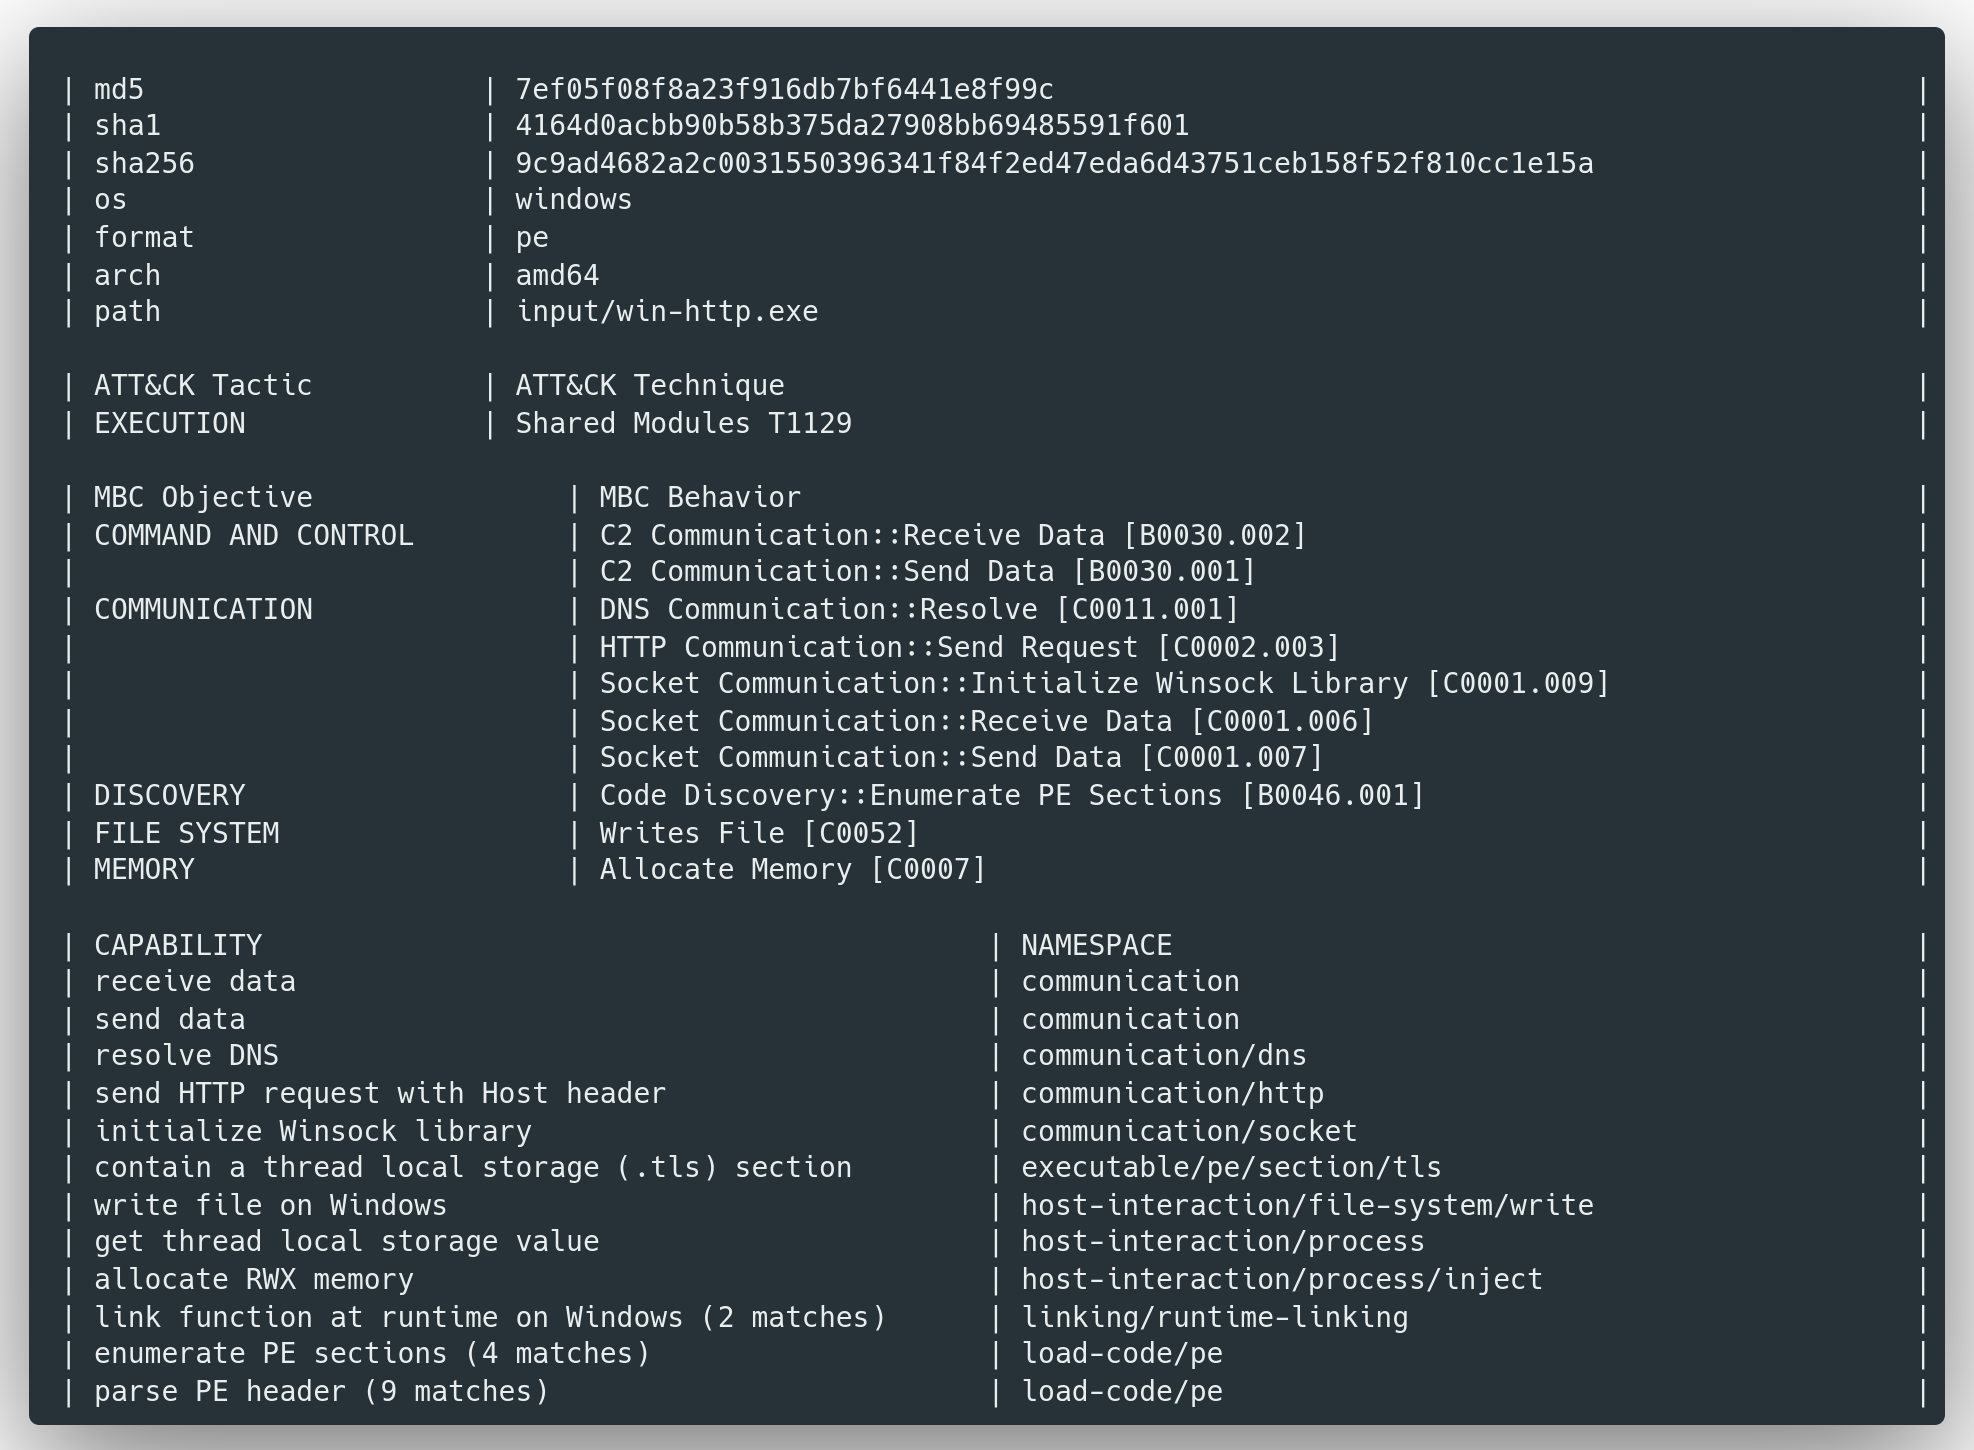
\includegraphics[width=0.75\textwidth]{assets/capa_out_first_parse.png}
    \caption{Prima trasformazione dell'output di capa}
    \label{fig:capa_out_first_parse}
\end{figure}

Possiamo stabilire una tecnica per ogni sezione, come segue:
\begin{itemize}
    \item \textbf{Info} potrà essere vista come un dizionario (chiave-valore) con come chiave il testo della prima colonna, e il valore preso dalla seconda colonna alla riga corrispondente;
    \item \textbf{Tactics} e \textbf{Objectives} possono essere viste entrambe come dizionari multi-valore, dove il valore è una lista -
    infatti, se una riga ha una chiave (prima colonna non vuota), creeremo una nuova lista di valori, altrimenti potrà essere appeso alla lista corrispondente alla chiave precedente
    \item \textbf{Capabilities} segue una logica analoga ma invertendo le colonne: qui la chiave è il namespace e come valore c'è la lista di capabilities stesse, con un maggiore parsing, che include sia il nome della capabilities che il numero di match (in figura \ref{fig:capa_out_first_parse} notiamo questa situazione nelle ultime 3 righe dell'output) 
\end{itemize}

In questo modo, si arriva ad un formato JSON machine-readable, che astrae dallo specifico formato di output di capa, che potrebbe cambiare tra major release, e allo stesso tempo organizzato in maniera sufficientemenete logica per essere consultato dall'analista di sicurezza nell'ambito del proprio studio del sample.

\begin{code}
\begin{minted}{json}
{
  "info": {
    "os": "windows",
    "format": "pe",
    "sha256": "9c9ad4682a2c0031550396341f84f2ed47eda6d43751ceb158f52f810cc1e15a"
  },
  "tactics": [{
    "tactic": "EXECUTION",
    "techniques": [ "Shared Modules T1129" ]
  }],
  "objectives": [{
    "objective": "COMMAND AND CONTROL",
    "behaviors": [
      "C2 Communication::Receive Data [B0030.002]",
      "C2 Communication::Send Data [B0030.001]"
    ]
  }],
  "capabilities": [{
    "namespace": "load-code/pe",
    "capabilities": [
      {
        "capability": "enumerate PE sections",
        "matches_count": 4
      },
      {
        "capability": "parse PE header",
        "matches_count": 9
      }
    ]
  }]
}
\end{minted}
\caption{Esempio sintetico del formato di output successivo al parsing}
\end{code}

%\newpage
\section{Riconoscitore custom del tipo di file}
\label{chap:static_custom_file_detector}
Partendo dalla necessità di velocizzare l'operazione di riconoscimento del file, in sostituzione dell'esecuzione del comando \texttt{capa -r anti-analysis} che può portare a richiedere diversi minuti a seconda del numero di funzioni presenti nel file, come visto in figura \ref{fig:capa_correlation_plot},
dobbiamo ricorrere a una diversa soluzione.

Dato che si tratta di un problema di enumerazione, non aveva senso andare a creare e mantenere un proprio riconoscitore di ogni possibile formato di un file. Ad esempio, già solo per quanto riguarda i file pacchettizzati, esistono tantissimi packer e tanti ne esisteranno in futuro.

Inoltre, spesso malware usano packer personalizzati, che hanno leggere differenze da quelli noti e si correrebbe il rischio di creare uno strumento poco efficace.
Per questi e altri motivi quali il tempo a disposizione, si era inizialmente scelto di usare come base uno strumento noto (\texttt{Detect-It-Easy}) per fare una prima analisi, affiancato da uno script Python custom che decide quali operazioni svolgere a seconda del tipo di file, va a fare il parsing del JSON dato in output e si integra nello script Bash creando un layer di astrazione col resto del workflow.
Infatti, nel caso servisse modificare lo strumento sottostante, sarebbe sufficiente adattare la traduzione dall'output specifico del tool al contratto stabilito col resto del programma per rendere seamless questa variazione, anche sostanziale.
Tuttavia, ci sono alcuni tipi che anche Detect-It-Easy fallisce a riconoscere, portando poi a un crash di capa quando eseguito.

Per questo motivo è stato creato un \textbf{custom detector}, scritto in Python, che implementa in maniera molto più efficiente e diretta, le sole regole di capa che riconoscono i file specifici su cui non è in grado di lavorare.

Di seguito possiamo osservare come funziona per dei tipi famosi di questi strumenti, ovvero il packer UPX e l'installer InnoSetup.
Sono state usate caratteristiche e regole note
\footnote{\url{https://github.com/mandiant/capa-rules/tree/e88db21de4d4cf9f7abec9177fab11240075036b/anti-analysis/packer}}
per eseguire la detection.

La lettura degli header del file PE sfrutta la libreria Python \texttt{pefile} per non eseguire l'intero parsing a mano dei byte degli header e non essere dipendenti da implementazioni native dell'OS come con l'uso dell'header \texttt{<windows.h>} in un programma C.

\begin{figure}[!htb]
    \centering
    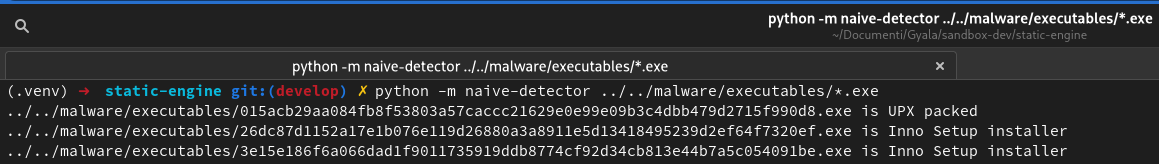
\includegraphics[width=\textwidth]{assets/custom_file_detector_output.png}
    \caption{Custom file detector output}
\end{figure}

\subsection{UPX}
Le regole più comuni
\footnote{\url{https://github.com/mandiant/capa-rules/blob/e88db21de4d4cf9f7abec9177fab11240075036b/anti-analysis/packer/upx/packed-with-upx.yml}}
per riconoscere UPX impongono di leggere le sezioni, e vedere se queste contengono \texttt{UPX0} o \texttt{UPX1}.

Facciamo una comparazione tra la regola capa per il rilevamento e il codice del riconoscitore.

\noindent\begin{minipage}{.35\textwidth}
       \begin{minted}{yaml}
features:
    - format: pe
    - or:
      - section: UPX0
      - section: UPX1
       \end{minted}
\end{minipage}
\begin{minipage}{.4\textwidth}
       \begin{minted}{python}
def is_upx(file_path):
    file_sections = get_section_names(file_path)
    upx_sections = [ "UPX0", "UPX1" ]
    for upx_section in upx_sections:
        if upx_section in file_sections:
            return True
    return False
       \end{minted}
\end{minipage}

\bigskip

Andando però a sfruttare la libreria Python per il parsing del file PE senza ricorrere a implementazioni native Windows:

\begin{minted}{python}
import pefile

def get_section_names(file_path):
    pe = pefile.PE(file_path)
    sections_set = {
        section.Name.decode().strip().strip('\x00')
        for section in pe.sections
    }
    pe.close()
    return sections_set
\end{minted}

\subsubsection{Analisi preliminare con readelf}
Notiamo come questa tecnica funzioni solo in ambito Windows, mentre su sistemi GNU/Linux notiamo con strumenti quali \texttt{readelf} che il file sia privo di header delle sezioni
(in accordo con la regola CAPA stessa, che infatti include questo match solo se ci troviamo su un file PE, come indicato dall'apposita riga \texttt{- format: pe}).

Negli eseguibili in formato ELF infatti è più comune trovare una situazione in cui l'header delle sezioni è mancante. Infatti, tale informazione non è usata in alcun modo dal kernel durante il caricamento in memoria del programma, nella creazione della process image. Inoltre, non è indicatore di azioni malevoli, ma sicuramente della volontà di rendere l'analisi più difficile, il cui caso può riguardare anche binari di produzione di software proprietario closed-source.

\subsubsection{Analisi dell'entropia}
Una caratteristica comune di binari compressi o con payload criptati è l'aumento di entropia. Infatti, sia la compressione che la crittografia vanno ad aumentare l'entropia all'interno di uno stesso blocco di file, motivo per cui è essenziale eseguire la compressione di un file prima della sua crittazione, altrimenti l'algoritmo di compressione sarebbe molto meno efficace.

Come esempio, è stato preso un eseguibile il cui sorgente è ininfluente, compilato con il compilatore C \texttt{gcc} e poi calcolata l'entropia sia prima che dopo averlo pacchettizzato con UPX. I grafici sono stati generati tramite l'ausilio di uno script Python creato ad-hoc e sfruttando il calcolo dell'entropia di Shanon.

\begin{figure}[htbp]
    \centering
    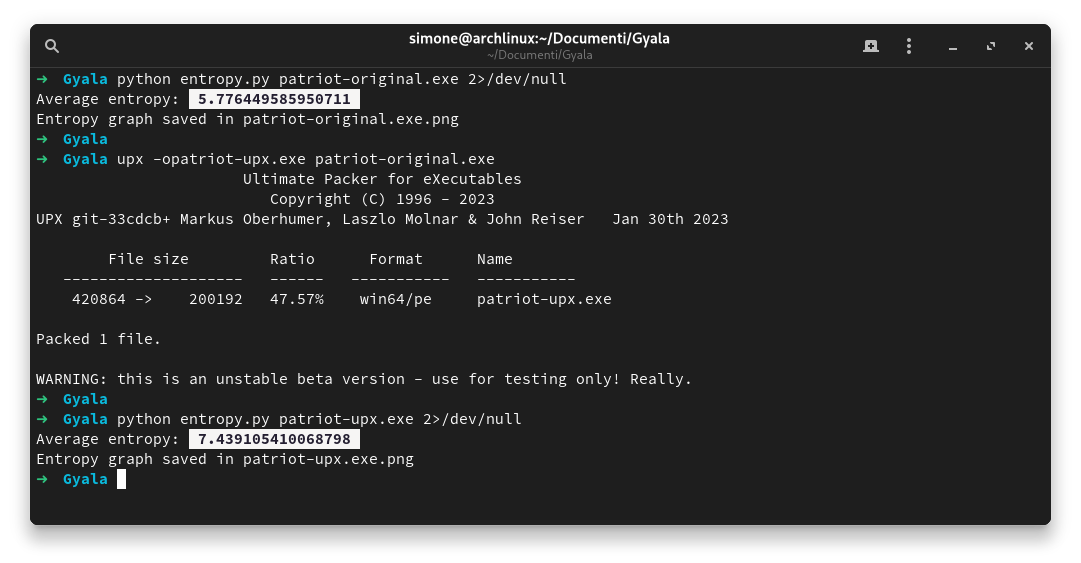
\includegraphics[width=0.75\textwidth]{assets/entropy_script_terminal.png}
    \caption{Esecuzione dello script per il calcolo dell'entropia e uso di UPX}
    \label{fig:entropy_script_terminal}
\end{figure}

\begin{figure}[!htb]
    \centering
    \begin{subfigure}[t]{0.48\textwidth}
        \centering
        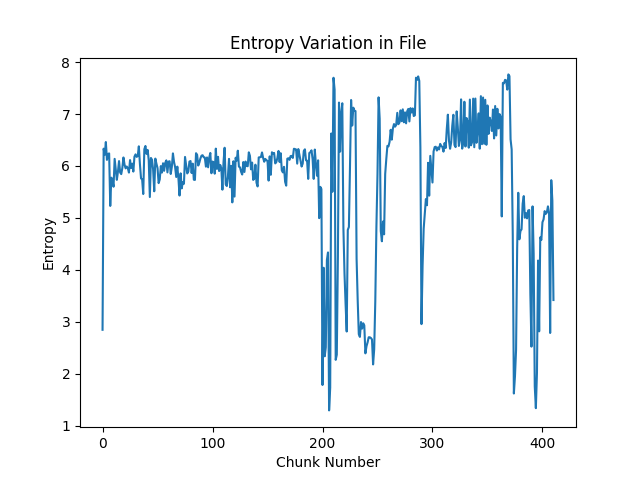
\includegraphics[width=\textwidth]{assets/patriot-original.exe.png}
        \caption{Entropia del file originale}
    \end{subfigure}
    \begin{subfigure}[t]{0.48\textwidth}
        \centering
        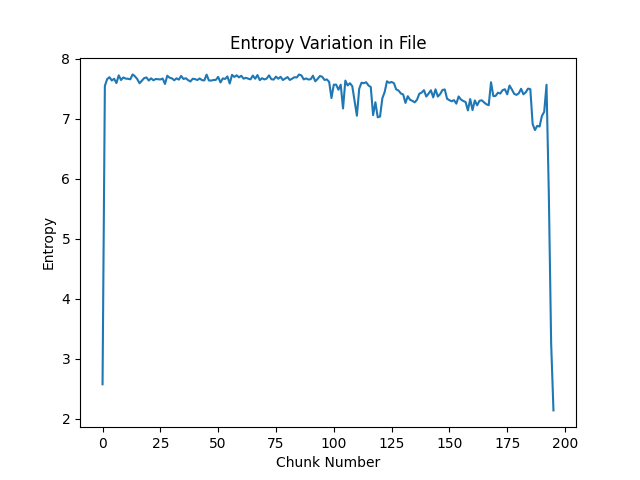
\includegraphics[width=\textwidth]{assets/patriot-upx.exe.png}
        \caption{Entropia del file pacchettizzato con UPX}
    \end{subfigure}
    \caption{Confronto dell'entropia prima e dopo l'uso di UPX}
    \label{fig:entropy_upx_comparison}
\end{figure}

\begin{figure}[htbp]
    \begin{subfigure}[t]{0,48\textwidth}
        \begin{gather*}
            H(x) = - \sum_{i=1}^{n} \frac{count_i}{N} \log{\left(\frac{count_i}{N}\right)}
        \end{gather*}
    \end{subfigure}
    \begin{subfigure}[t]{0,48\textwidth}
        \begin{minted}{python}
def calculate_entropy(data):
    entropy, size = 0, len(data)
    if size <= 1: return entropy

    byte_count = [0] * 256
    for byte in data:
        byte_count[byte] += 1

    for count in byte_count:
        if count > 0:
            probability = float(count) / size
            entropy -= probability \
                * math.log(probability, 2)

    return entropy
        \end{minted}
    \end{subfigure}
    \caption{Formula dell'entropia di Shannon e codice Python per il calcolo su un chunk}
    \label{fig:shannon_entropy_formula}
\end{figure}

%%%%%%%%%%%%% http://blog.dkbza.org/2007/05/scanning-data-for-entropy-anomalies.html
%%%%%%%%%%%%% https://fsec404.github.io/blog/Shanon-entropy/

\subsection{Inno-Setup Installer}
Con Inno-Setup, possiamo notare come sia ancora più semplice il riconoscimento. Infatti, non abbiamo bisogno di andare a vedere le sezioni, ma è sufficiente controllare la presenza di alcune stringhe statiche nel file.

InnoSetup è un famosissimo installer per Windows e, come tale, non permette un'analisi statica
efficace. Infatti, nulla vieta che appaia come lecito per poi andare a runtime a scaricare e installare il vero payload malevolo, ma tale comportamento è affidato alla parte dinamica dell'analisi, dove sarà possibile osservare anche tutti i file scaricati, oltre all'attività di rete e tutte le syscall richiamate.

Nuovamente, andiamo a paragonare la regola capa alla nostra implementazione:

\begin{minipage}{\textwidth}
\begin{minted}{yaml}
features:
    - and:
      - string: /^Inno Setup Setup Data \(/
      - string: /^Inno Setup Messages \(/
\end{minted}

\begin{minted}{python}
def is_innosetup(file_path):
    BUFFER_SIZE = 65536
    with open(file_path, 'br') as f:
        match_setup, match_messages = False, False
        buffer = f.read(BUFFER_SIZE)
        overlap = len(b'Inno Setup Setup Data (')

        while len(buffer) > overlap and (not match_setup or not match_messages):
            # Match inside current buffer
            if not match_setup and b'Inno Setup Setup Data (' in buffer:
                match_setup = True
            if not match_messages and b'Inno Setup Messages (' in buffer:
                match_messages = True
            
            # Read next buffer, allowing for overlap
            buffer = buffer[-overlap:] + f.read(BUFFER_SIZE)
    
    return match_setup and match_messages
\end{minted}
\end{minipage}

\subsection{Design scalabile e modulare}
Si nota immediatamente come una tale implementazione è poco scalabile e presenta numerose ridondanze da rimuovere.

Studiando le regole di interesse all'interno del repository GitHub \textit{capa-rules}, osserviamo come le regole siano principalmente di due categorie: basate su match di stringhe o basate su match di nomi di sezioni nel file eseguibile.

Da questa osservazione, elaboriamo la struttura del programma software di detection. Precisamente, decidiamo di strutturarlo in classi dove ogni regola è una classe a sé, e individuiamo le seguenti classi padre (figura \ref{fig:base_custom_static_analyzer_uml}):
\begin{itemize}
    \item \texttt{BaseRule} conterrà le logiche di base che possiede una regola, tra cui un getter per il nome e un metodo \texttt{match()}
    \item \texttt{StringRule} conterrà il codice unico per tutte le regole che basano il loro match sulla presenza di determinate stringhe all'interno del file, quindi la classe figlia dovrà solo fornire le stringhe da cercare e la logica di match (ad esempio: tutte le stringhe richieste devono essere state trovate = and logico; una sola stringa trovata è sufficiente = or logico)
    \item \texttt{SectionRule} analogamente a prima conterrà le procedure di estrazione delle sezioni dal file, con la logica di match nelle classi figlie, ossia le effettive regole.
\end{itemize}

Sempre al fine di ottimizzare i tempi di esecuzione di questo rilevamento statico sul file eseguibile,
andiamo a creare una classe wrapper sopra \texttt{pathlib.Path} che esporrà i metodi per leggere le sezioni, procedura lenta se ripetuta per ogni singola regola, e alcune altre funzioni di utilità come la rilevazione del tipo basilare di file (PE o ELF) eseguibile tramite l'ausilio di \texttt{libmagic}, la stessa che permette al comando \texttt{file} di operare.
Quindi da un lato è stata aumentata l'astrazione tra la business logic del programma e i dettagli implementativi delle librerie sottostanti, dall'altro possiamo aggiungere meccanismi di lazy-loading e caching di tali informazioni richieste.

\begin{figure}[H]
    \centering
    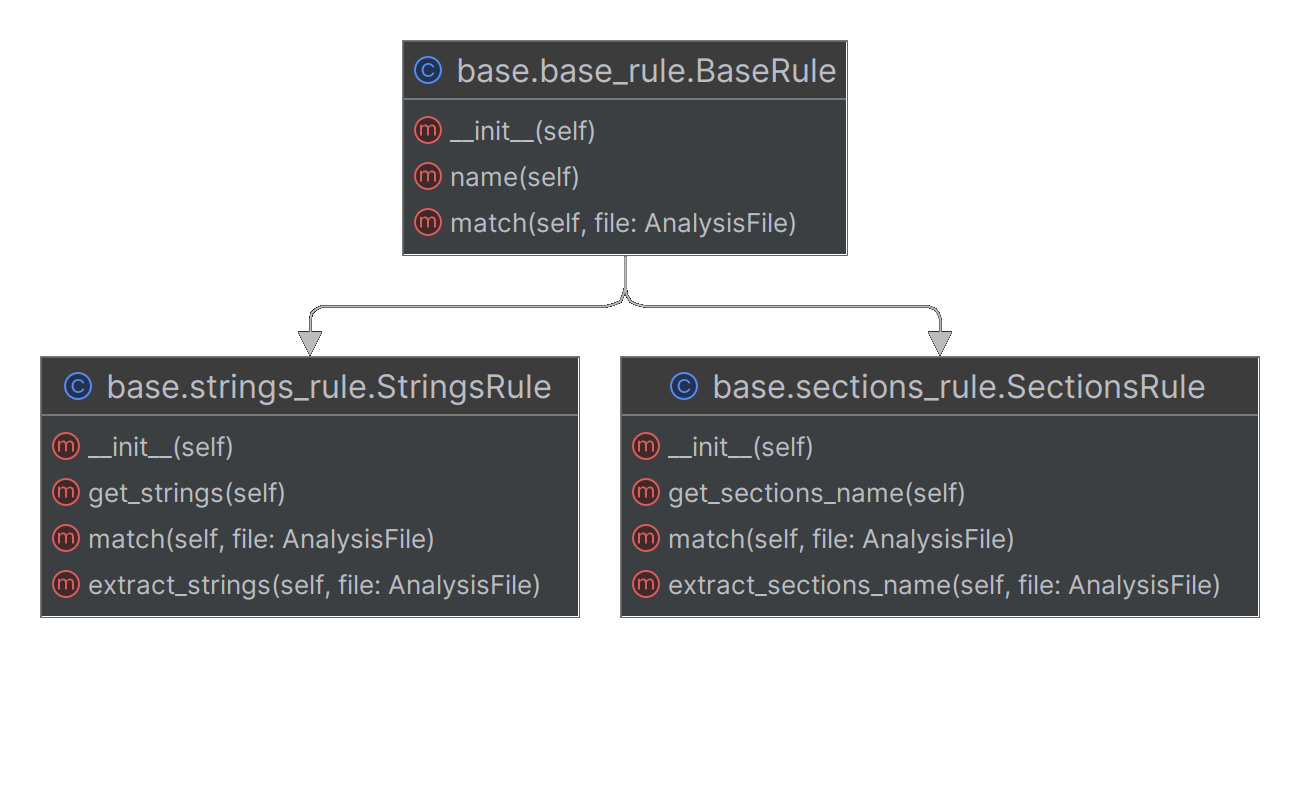
\includegraphics[width = 0.8\textwidth]{assets/base_custom_static_analyzer.png}
    \caption{Diagramma UML delle classi}
    \label{fig:base_custom_static_analyzer_uml}
\end{figure}

\begin{code}
    \begin{minted}[samepage]{python}
class InnoSetupDetector(StringsRule):
    def name(self) -> str:
        return 'executable/installer/inno-setup'

    def get_strings(self) -> list[bytes]:
        return [
            b'Inno Setup Setup Data (',
            b'Inno Setup Messages (',
        ]

    def match(self, file: AnalysisFile) -> bool:
        # && logic
        return len(self.extract_strings(file)) == len(self.strings)
    \end{minted}
    \caption{Regola di riconoscimento di InnoSetup, usando la nuova architettura}
    \label{code:innosetup_custom_recognizer}
\end{code}

\section{Yara: signature-based}
Un altro strumento adoperato per una più ampia analisi statica del file è Yara.
Questo tool utilizza le cosiddette \emph{Yara rule} per descrivere una regola ed eseguire così signature matching.

\begin{code}
    \begin{minted}[samepage]{yaml}
rule ExampleRule
{
    strings:
        $my_text_string = "text here"
        $my_hex_string = { E2 34 A1 C8 23 FB }

    condition:
        $my_text_string or $my_hex_string
}
    \end{minted}
    \caption{Regola di Yara di esempio}
    \label{code:yara_example_rule}
\end{code}

Nella regola di esempio (listing \ref{code:yara_example_rule}) possiamo osservare nel blocco \emph{strings} le stringhe, o la regex, che di cui vogliamo fare il match, e successivamente la condizione per dare esito positivo alla regola.

Questo strumento è ampiamente usato nell'ambito della malware analysis sia su file staticamente che durante la loro esecuzione per fare matching sulla memoria dei processi. Tuttavia, nello scopo del progetto viene relegato all'uso su base statica.

\subsection{Collezione delle regole}
Al contrario di capa (visto nella sez. \ref{chap:capa}), questo tool non viene fornito di un set di regole predefinite, ma dobbiamo andare a collezionarle autonomamente.
Tuttavia, essendo molto famoso, si trovano facilmente repository di professionisti e aziende di rilievo che scelgono di rendere le loro regole disponibili alla community. Bisogna però notare come non tutte le regole siano di qualità e potrebbero in alcuni casi essere controproducenti, generando una quantità eccessiva di falsi positivi o non essere aggiornate o sufficientemente generalizzate da creare falsi negativi.
A questo scopo, viene usato lo strumento di \emph{Retrohunt} di VirusTotal Enterprise, che permette di sapere anticipatamente quanti file fanno il match con una data regola, andando a usare l'ampissimo database di VirusTotal. In questo modo, se vedremo un numero troppo elevato di match, probabilmente la regola genera falsi positivi, con un discorso speculare in casi di troppi pochi match.

I principali repository di regole Yara sono di Florian Roth
\footnote{\url{https://github.com/Neo23x0/signature-base}}
nonché di Apple per quanto concerne MacOS e altre fonti autorevoli in materia.

Per ridurre l'esecuzione di regole inutili, viene sfruttato il rilevamento del sistema operativo precedentemente messo in opera per andare ad eseguire solo regole che abbiano quell'OS come target.
Allo scopo, le regole sono mantenute in locale e nell'analizzatore divise in cartelle:
\begin{itemize}
    \item \emph{windows, macos, linux} a seconda del sistema operativo target
    \item \emph{common} se sono state ritenute di uso generale per cui ha senso eseguirle in ogni caso, qualunque sia il tipo di file sotto analisi
    \item \emph{unclassified} conterrà regole che ancora non sono state catalogate da parte dell'analista, ma si ha la necessità di integrarle al momento nel tool, eseguendole sempre; differisce da "common" per il fatto che queste regole potrebbero riguardare anche un solo OS ma temporaneamente le eseguiamo sempre - non possono essere inserite temporaneamente in "common" per una questione di ordine
\end{itemize}

\section{Fuzzy hashing}
In un'ottica di uso su larga scale, è coerente con le esigenze aziendali avere un sistema di comparazione dei sample. Uno dei modi più semplici ma robusti per eseguire tale confronto è il fuzzy hashing. Questa tecnica consiste nel creare un hash del file che, al contrario di quanto accade nelle funzioni di hashing tradizionali come SHA-256 dove anche una minima modifica al file va a generare un hash completamente diverso, qui la differenza nell'impronta hash è commisurata alle modifiche in un dato file. Ne consegue che file simili, dove è cambiato poco, come una costante o un IoC qualsiasi, avranno un fuzzy hash molto simile.

Una delle funzioni più famose è \textbf{SSDeep}.
In figura \ref{fig:ssdeep_demo_run} è stato creato un file random e una sua versione modificata alterando i primi 8 Byte: possiamo notare come solo il primo carattere sia modificato, di fatto riflettendo una modifica solo nella prima porzione di file. Al contrario, notiamo come un hashing come SHA256 presenta numerosissime modifiche, essendo indicato per tutt'altro scopo.

\begin{figure}[htbp]
    \centering
    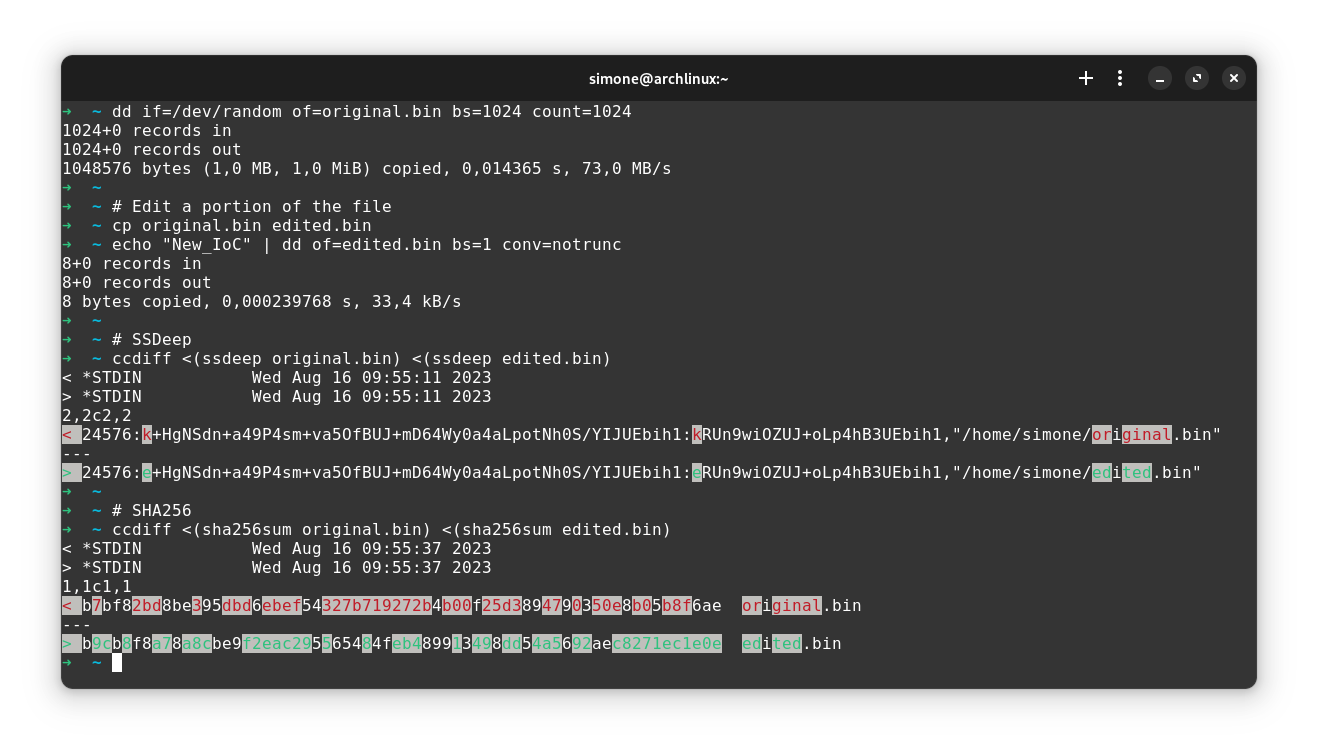
\includegraphics[width=0.9\textwidth]{assets/ssdeep_demo_run.png}
    \caption{Esempio di fuzzy hashing tra file con solo alcuni byte modificati}
    \label{fig:ssdeep_demo_run}
\end{figure}

In questo modo, possiamo lanciare una funzione di distanza tra stringhe e calcolando il numero di caratteri dell'hash diversi, stabilire un grado di somiglianza con altri sample noti. Nel caso di un malware mai visto prima, potremo in realtà scoprire che si tratti solamente di una versione modificata di un sample già nel nostro archivio, facendo risparmiare una quantità di lavoro e accellerando i processi.

Il suo funzionamento è intuibile dal formato dell'impronta ottenuta. Si tratta di un \emph{Context-Triggered Piecewise Hash} ed è prodotto andando ad eseguire una funzione hash su ogni porzione di file di dimensione fissata, indicata nella prima parte. Seguono hash per ogni porzione, permettendo di capire chiaramente dove è situata la modifica. Inoltre, è relativamente resistente anche a zero padding, in cui l'attaccante potrebbe pensare di inserire nel payload un numero importante di zero per cercare di rendere più differenti posssibili i due sample.

\section{Strumenti minori}
A dimostrazione della flessibilità dello strumento realizzato, sono stati integrati altri due strumenti importanti ma di minor rilievo rispetto a quelli appena enunciati.

\begin{itemize}
    \item \textbf{Detect-It-Easy}: permette di identificare il tipo di un file eseguendo un'analisi più profonda di quanto faccia \texttt{libmagic}, utilizzabile dall'utente attraverso il comando \texttt{file} su sistemi Unix, includendo tutta una serie di metadati come il tipo di installer presente, il linker usato, o altre informazioni di questo tipo
    \item \textbf{ExifTool}: un tool Perl in grado di estrarre un gran numero di metadati in una varietà di formati di file, oltre agli eseguibili, incluse foto, PDF, file Office, e così via
\end{itemize}

\begin{code}
\begin{minted}{json}
{
    "diec": {
        "arch": "AMD64",
        "detects": [{
            "name": "unknown",
            "options": "Console64,console",
            "string": "linker: unknown(2.38)[Console64,console]",
            "type": "linker",
            "version": "2.38"
        }],
        "endianess": "LE",
        "filetype": "PE64",
        "mode": "64",
        "type": "Console"
    },
    "exiftool": {
        "ExifToolVersion": 12.62,
        "FileType": "Win64 EXE",
        "MachineType": "AMD AMD64",
        "ImageFileCharacteristics": "Executable, No line numbers, No symbols, ...",
        "CodeSize": 47616,
        "InitializedDataSize": 122368,
        "UninitializedDataSize": 5120,
        "EntryPoint": "0x14d0",
        "SubsystemVersion": 5.2,
        "Subsystem": "Windows command line",
        "ProductVersionNumber": "0.6.0.0",
        "ObjectFileType": "Executable application",
        "LanguageCode": "English (U.S.)",
        "CharacterSet": "Windows, Latin1",
        "FileDescription": "Paranoid Fish is paranoid",
        "ProductName": "Paranoid Fish"
    }
}
\end{minted}
\caption{Output parziale dei dati ottenuti dai due strumenti minori}
\end{code}

\section{Containerizzazione}
Al fine di utilizzare tutti questi strumenti in una maniera organizzata e flessibile,
si arriva alla necessità di avere un sistema unico e portatile tra vari sistemi per l'esecuzione. La soluzione migliore a tale scopo è usare un Container Docker.
Questo permette di avere un certo livello di isolamento tra lo strumento di analisi e il sistema host sul quale è realmente eseguito, senza tutti gli overhead che comporta una macchina virtuale. Inoltre, possiamo avviarlo a piacimento fornendo direttamente un input da analizzare, montando una cartella come volume read-only, e far si che si elimini automaticamente dopo la sua esecuzione.
Dato lo scopo e l'ambito di applicazione del progetto, usare un container permetterà di eseguire il tutto in maniera più semplice possibile su Amazon Web Services (di seguito, AWS).

\subsection{Flusso di esecuzione}
Viene così costruito un chiaro flusso di esecuzione dei vari strumenti, parser e componenti accessorie realizzate, inclusa una chiara gestione degli errori e loro propagazione all'esterno in maniera documentata, al fine di avere una chiara integrazione con gli altri strumenti, quali FSL menzionato nell'introduzione al capitolo \ref{chap:intro_interface_with_other_services}. L'intero flusso è implementato attraverso uno \textbf{script sh} che controlla le condizioni dei vari tool in caso debbano essere gestite, o termina l'esecuzione propagando l'exit code allo script richiamante attraverso il flag \texttt{set -e} posto all'inizio.
Viene usato \texttt{/bin/sh} come interprete anziché \texttt{/bin/bash} per ridurre la superficie di attacco in caso di future vulnerabilità in qualche strumento, o evitare di introdurne noi alcune date dalla grande varietà di funzionalità offerte da bash e di cui non abbbiamo alcun bisogno.

Per prima cosa, si è deciso di eseguire Detect-It-Easy per avere una prima idea, seppur non comprensiva di tutti i casi limite di capa, del tipo di file che stiamo per analizzare. Il suo output viene salvato in un file JSON associato, che verrà consegnato al termine dell'analisi, ma da cui vengono estratte le prime informazioni essenziali per il resto del flusso, tra cui il sistema operativo e il tipo di file (PE, ELF, ...).

Già da qui, se il file non viene rilevato come PE o ELF, andiamo a saltare l'esecuzione di \texttt{capa} che sicuramente condurrà ad un errore.
Per coprire anche tutti gli altri casi precedentemente discussi, dobbiamo eseguire l'analizzatore statico costruito ad-hoc (sez. \ref{chap:static_custom_file_detector}). Questo andrà a controllare con molta più accuratezza se è un tipo di eseguibile supportato,
controllando sia le situazioni descritte da alcune regole capa che l'architettura dato che è compatibile solo con x86 e x86\_64.

Se ci troviamo in una situazione compatibile, viene eseguito \texttt{capa}. Questo è lo strumento più potente ma anche il più lento ed esoso di risorse, sia in termini di spazio che di tempo. Siccome è il più probabile al crash, viene gestito il suo exit-code fallimentare con un error message diverso dagli altri, per restituire al termine dell'esecuzione più informazioni possibili di debug e diagnostica, oltre ai log che però non sono direttamente inclusi nel file di risultato finale di analisi, ma dovranno essere collezionati separatamente.
Come annunciato, l'output testuale di capa viene inviato al parser con una pipe, il quale darà in output il JSON risultante.

Dopodicché si prosegue con l'esecuzione dell'altro importante strumento: \texttt{yara}. Offre la possibilità di indicare a runtime quali set di regole eseguire. Ricordiamo di aver provveduto alla divisione delle regole collezionate in collezioni per sistema operativo, quindi leggendo il sistema operativo precedentemente identificato, possiamo specificare quale collezione usare. In caso non si tratti di un eseguibile o sia un sistema operativo sconosciuto / non considerato, verranno eseguite tutte le regole in quanto i rischi di perdere informazioni utili in questo caso supererebbero i benefici del risparmio di regole.

Infine, procediamo con l'esecuzione di strumenti quali ExifTool e fuzzy hashing con ssdeep.
Tutti gli strumenti avranno così dato in output i propri risultati nel proprio file JSON. In conclusione, viene invocato un altro script Python che si occuperà di eseguire una validazione sintattica di tutti i risultati e, in caso di successo, eliminerà i file parziali per restituire l'unico report JSON complessivo di tutto.
Questo ultimo layer di astrazione è utile sia per unificare i risultati intermedi che per avere la possibilità di modificare gli strumenti sottostanti con analoghi, potendo sfruttare questo ultimo passaggio per uniformare il formato dell'output così da rendere il tutto trasparente al chiamante.

\begin{figure}[htbp]
    \centering
    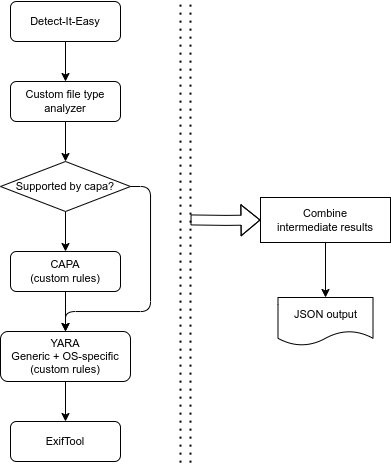
\includegraphics[width=0.75\textwidth]{assets/static_run_analysis_internal_tools.png}
    \caption{Workflow processo interno di \texttt{run\_analysis}}
    \label{fig:static_analysis_internal_tools_workflow}
\end{figure}

\subsection{Efficienza delle regole}
Noto che ad ogni esecuzione di un'immagine Docker all'interno di un ambiente containerizzato, il container finale verrà distrutto, ci si è resi conto di come alcune regole vedano sempre una precompilazione o caching ad ogni invocazione, quando sarebbe idealmente più ottimale eseguire questo step una sola volta.
Dopo uno studio più approfondito di questi strumenti, è emerso come i due principali (ossia \texttt{capa} e \texttt{yara}) abbiano modi per eseguire questo step in anticipo.

Per quanto concerne capa, successivamente aver analizzato il proprio processo di CI/CD
\footnote{\url{https://github.com/mandiant/capa/blob/master/.github/workflows/build.yml}}
disponibile nel repository GitHub da cui è possibile scaricarlo precompilato od ottenere il sorgente, ci si è resi conto che questo processo sarebbe stato realizzabile.
Nel processo di build della nostra immagine Docker viene ora inserito un passaggio che permetta di:
\begin{itemize}
    \item Clonare il repository GitHub di capa
    \item Eseguire il checkout del repository e dei propri submodules alla versione fissata, così da rendere la build al massimo replicabile in futuro
    \item Inserire le regole personalizzate, rimuovendo le predefinite
    \item Eseguire un caching delle regole ahead-of-time, come nel processo ufficiale di CI/CD
    \item Ora poter compilare il nostro eseguibile di capa e usarlo nelle varie esecuzioni al posto del precompilato già disponibile
\end{itemize}

In secondo luogo, occupandoci anche del tool \texttt{yara}, si è visto come disponga di API Python che ne permettono l'uso. Seguendo la documentazione ufficiale, offre la possibilità di salvare su file la versione precompilata delle regole.
Così, analogamente a quanto appena visto, è stato inserito uno step aggiuntivo nella build che prenda le regole personalizzate, esegua queste funzioni da uno script Python, salvando i file precompilati senza dover conservare anche le regole originali, avendo tuttavia cura di mantenere la struttura delle cartelle inalterata.

Queste modifiche hanno permesso di rendere le esecuzioni più veloci di un tempo al momento trascurabile, ma che porterà maggiori benefici in futuro, quando il numero delle regole diventerà sostanzialmente più elevato, eseguendo uno step solo al momento di build e non ad ogni esecuzione.

\subsection{Multi-stage build}
Rimanendo in tema di build dell'immagine Docker, ci si rende subito conto come l'immagine prodotta in maniera naive abbia dimensioni di $>2$ GB. Essendo una dimensione non giustificabile dalla presenza di strumenti troppo pesanti, si è reso necessario trasformare il Dockerfile per utilizzare una metodologia multi-stage.
Questa tecnica permette di generare e lavorare su tante immagini diverse, ad esempio per eseguire compilazioni, copiare codici sorgente, installare software di compilazione pesante poi mai più usato in fase di esecuzione, per poi distribuire solo l'ultima di questa serie di immagini, che dovrebbe ottimalmente contenere solo lo stretto indispensabile per una corretta esecuzione, rimuovendo il superfluo che resta nelle immagini intermedie non distribuite.

Dividiamo il processo di build in vari step logici, avendo sempre cura di fissare l'hash delle immagini usate dal registry Docker Hub, così da avere la certezza di poter riprodurre la build anche in futuro e anche in caso di modifica/aggiornamento delle immagini corrispondenti a un dato tag:
\begin{enumerate}
    \item Partendo da una immagine Debian 12, installiamo python, pip e tutte le altre dipendenze richieste a tempo di compilazione o utilità come git
    \item Nell'immagine di Python così ottenuta, creiamo un nuovo virtualenv e impostiamo le necessarie variabili d'ambiente; riguardo al virtualenv ricordiamo come non sia possibile eseguire lo script \texttt{.venv/bin/activate} come si farebbe normalmente su un sistema interattivo, perché ogni comando \texttt{RUN} in un Dockerfile esegue su una shell diversa, quindi dobbiamo modificare \texttt{PATH} e \texttt{PYTHONPATH} per puntare all'interno del virtualenv
    \item In un'immagine, andiamo a clonare capa da GitHub, eseguire il checkout alla versione desiderata attraverso il tag di git e costruire l'eseguibile come precedentemente illustrato
    \item Parallelamente, creiamo un'immagine che conterrà molte più dipendenze di build su cui andremo ad installare yara ed eseguire la precompilazione delle regole
    \item Ripartendo da un'immagine Debian 12 slim pulita, installiamo solo Python e le librerie strettamente necessarie a runtime
    \item Su questa, installiamo i tool secondari, come Detect-It-Easy o ExifTool che non richiedono passaggi aggiuntivi se non il download di un file
    \item In conclusione, verrà copiato il codice sorgente del progetto realizzato e distribuita quest'ultima immagine
    \item Esiste anche uno step di test preliminare, dove viene controllato che i comandi esistano nel \texttt{PATH} e poco altro, visto che i test funzionali veri e propri non sono inclusi nel Dockerfile, come dovrebbe essere da best practises
\end{enumerate}

Possiamo notare in figura \ref{fig:static_dockerfile_multistage_build} come il processo di build ad un certo punto si divida tra la precompilazione di capa e di yara. Sfruttando il più recente comando \texttt{docker buildx} al posto dell'ormai deprecato \texttt{docker build} possiamo ridurre i tempi di build dell'immagine finale di vari minuti, variabili a seconda del sistema su cui si esegue la build, ma pur sempre un gran risparmio di tempo ottenuto grazie all'effettiva parallelizzazione dei due branch.

\begin{figure}[htbp]
    \centering
    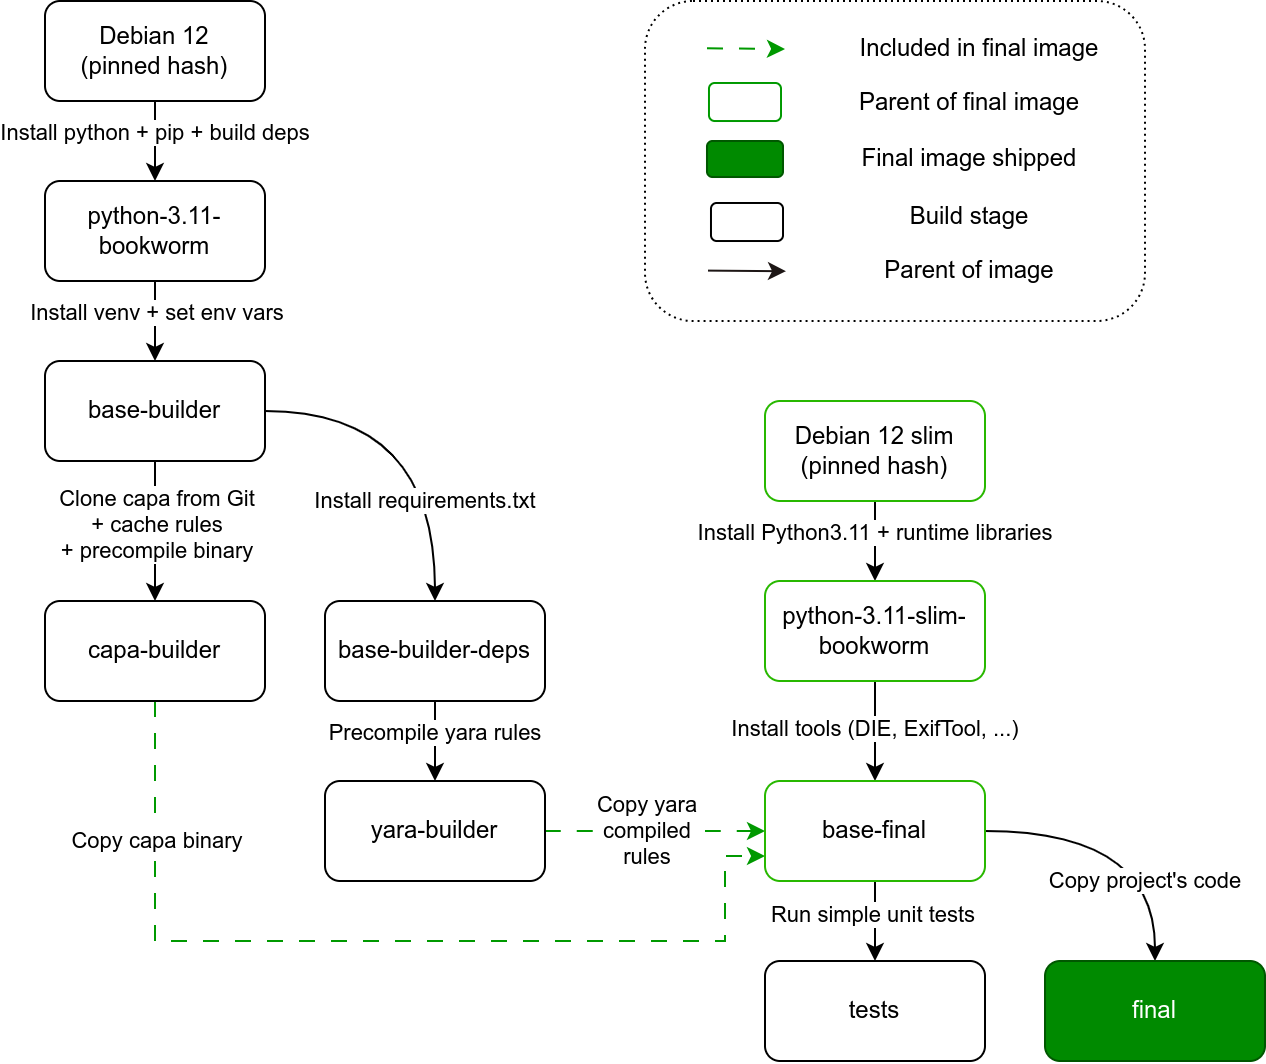
\includegraphics[width=\textwidth]{assets/dockerfile.png}
    \caption{Docker multi-stage build, con le immagini intermedie}
    \label{fig:static_dockerfile_multistage_build}
\end{figure}

\subsection{Entrypoint e flessibilità}
Come già annunciato, una delle linee guida mantenute a mente per l'intero progetto è quella della massima flessibilità degli strumenti creati. Qui vediamo una sua prima applicazione pratica.
Un'immagine Docker ha due proprietà distinte ma poco frequentemente adoperate: \texttt{ENTRYPOINT} e \texttt{CMD}.
L'entrypoint è quel comando che viene sempre eseguito all'avvio di un'immagine Docker e permette di eseguire una prima inizializzazione, come creare qualche cartella mancante, fare dei check di avvio essenziali o cambiare utente. Di default, un'immagine ha entrypoint \texttt{/bin/sh -c} e nessun comando specificato.
Il comando realmente eseguito è l'entrypoint, ricevendo come argomento il CMD. Com'è subito possibile notare dal flag \texttt{-c}, nel caso del default entrypoint, questo non farà altro che eseguire i comandi usando la shell \texttt{/bin/sh}.

Nel caso specifico di questo progetto, la divisione tra entrypoint e cmd viene notevolmente in aiuto nei casi in cui ci aspettiamo di avere vari utilizzi (implementati attraverso più cmd) ma vogliamo raccogliere a fattor comune le prime inizializzazioni obbligatorie (un unico entrypoint).
L'entrypoint ora costruito, andrà ad eseguire varie operazioni di bootstrap come controllare se sta eseguendo all'interno di una runtime AWS Lambda o su un sistema Docker tradizionale, creare la cartella di output se non esistente e proseguire l'esecuzione con un utente non privilegiato, siccome su un ambiente Docker tradizionale è comune che vengano eseguite come root, non gradito nel nostro ambito. Seppur non è come eseguire come root nel sistema host, essere root in un container è comunque un eccesso di privilegi rispetto al minimo indispensabile.
Ciò che deve essere eseguito è definito dal CMD che andrà a ricevere come argomento (essendo uno script, lo leggerà nella variabile "\texttt{\$@}").

Al momento, sono realizzati vari script da usare come cmd a seconda del caso d'uso specifico:
\begin{itemize}
    \item \texttt{analyze\_multiple.sh} si aspetta di ricevere l'insieme dei file da analizzare nella cartella montata nella posizione di input, procedendo a scrivere i JSON risultanti nella cartella di output seguendo la struttura di directory dell'input;
    \item \texttt{download\_and\_analyze.sh} si aspetta di ricevere come argomento un URL da cui scaricare con \texttt{wget} il sample da analizzare - è utile sia nei casi in cui non vogliamo far transitare il sample sul filesystem del sistema host, ma anche nel caso di AWS come vedremo nella prossima sezione
\end{itemize}

Il cmd viene specificato agevolmente al momento dell'esecuzione e corrisponde agli argomenti passati al comando \texttt{docker run} successivamente al nome dell'immagine. A titolo esemplificativo, se il comando eseguito è:
\texttt{docker run -it -rm -v /home/simone/output:/app/output static-engine:latest} \\ \texttt{/app/src/download\_and\_analyze.sh https://example.com/malware.bin}
lo script di entrypoint verrà eseguito ricevendo come argomenti il cmd, composto dallo script di download e analisi, nonché dall'URL del malware, che sarà successivamente l'argomento ricevuto da quest'ultimo script.

\section{Automazione su AWS}
\subsection{Architettura serverless}
Per architettura serverless si intende un particolare tipo di soluzione ingegneristica dove si procede a creare ed eseguire software senza l'onere di gestire l'infrastruttura sottostante, come ad esempio gestire il proprio server fisico, configurarlo e mantenerlo aggiornato nel tempo. Questo permette un risparmio di tempo ed è meno error-prone se non si hanno figure professionali specializzate dedicate. Ad oggi è generalmente la soluzione da preferire nella maggioranza delle situazioni in termini di costo-opportunità.
L'architettura è ben riassunta in figura \ref{fig:aws_static_lambdas_architecture} e si basa sul paradigma \emph{FaaS} (Function-as-a-Service), di seguito spiegata, dove l'entità principale della computazione è una funzione.

Il flusso di esecuzione ha inizio con l'upload del sample su un bucket S3
\footnote{S3 è un servizio di AWS che si occupa di object storage, un tipo di storage di file dove ciascuno è visto come un nome con il proprio contenuto in byte, metadati e poche altre informazioni - il nome S3 è acronimo di Simple Storage Service}
che ha lo scopo di archiviare tutti i sample da analizzati o che sono stati analizzati, per costruire un proprio repository interno di sample, maligni o meno che siano.
Su questo bucket è previsto che proceda al caricamento il componente aziendale FSL, parte dell'area di Threat Intelligence. Tuttavia, siccome non è ancora sviluppato ma è solo in programma, a fini di test e utilizzo iniziale, l'upload viene effettuato manualmente dalla console AWS, visto che non comporta alcuna differenza nel resto del processo.
L'upload andrà così ad eseguire il trigger dell'evento \texttt{ObjectCreated:Put}, ascoltato dalla prima delle 3 lambda coinvolte. Bisogna prestare attenzione al fatto di dover ascoltare sia l'evento Put che \texttt{ObjectCreated:CompleteMultipartUpload} visto che in caso di caricamento di file grandi, verrà invocato solo l'ultimo evento. Se non fosse ascoltato, non verrebbe mai scatenata la prima lambda e, di conseguenza, tutto il resto dell'analisi verrebbe meno.

La scelta architetturale di dividere l'esecuzione in 3 lambda anziché lasciar svolgere tutti i task a una sola Lambda, risiede nel voler minimizzare i permessi concessi alla fase di analisi. Seppur si tratta di un processo statico, quindi non prevede esecuzione del sample, non è in alcuna maniera escludibile una vulnerabilità di tipo RCE (Remote Code Execution) all'interno degli strumenti adoperati, o che verranno aggiunti successivamente,
ma è anzi più frequente di quanto ci si possa aspettare, e la superficie di attacco tende ad aumentare in maniera direttamente proporzionale al numero e alla complessità dei tool adoperati.

Al contrario, con questa soluzione, è stato possibile ridurre i permessi della fase di analisi, dove il contenuto del sample viene interpretato e non semplicemente trasferito sotto forma di byte o URL, ritenuto il momento più critico nell'intero processo. Può solamente:
\begin{itemize}
    \item Scrivere nelle proprie tracce di log su CloudWatch
    \item Invocare unicamente la Lambda a sè successiva
    \item Leggere solo il sample che deve analizzare
\end{itemize}

\noindent Non può quindi:
\begin{itemize}
    \item Accedere al bucket S3 per intero, prevenendo fughe di dati
    \item Accedere al servizio della Threat Intelligence che conserva i dati sulle analisi e i loro risultati
\end{itemize}

\begin{code}
\begin{minted}{json}
{
    "Version": "2012-10-17",
    "Statement": [{
        "Effect": "Allow",
        "Action": [
            "logs:PutLogEvents",
            "logs:CreateLogGroup",
            "logs:CreateLogStream"
        ],
        "Resource": "arn:aws:logs:*:*:*"
    },
    {
        "Effect": "Allow",
        "Action": [ "lambda:InvokeFunction" ],
        "Resource": "<static_analysis_reporting ARN>"
    }]
}
\end{minted}
\label{code:aws_static_analysis_lambda_policy}
\caption{JSON della policy assegnata alla Lambda dell'analisi}
\end{code}

Le policy assegnate alle varie entità su AWS sono state scritte da zero, mantenendo chiara la politica del minimo permesso concesso; sono state ritenute eccessivamente permissive le policy gestite fornite direttamente da AWS.

\medskip

La prima Lambda, chiamata \texttt{trigger\_new\_malware}, si occupa di ricevere l'evento invocato al termine dell'upload, quindi estrarre quali siano i nuovi file caricati, per ciascuno generare un \textbf{pre-signed URL} così da permettere la lettura del singolo oggetto per un periodo di tempo limitato e senza concedere permessi di lettura del bucket a terze entità.
Andrà quindi a invocare in maniera asincrona la lambda di analisi, inviando nel payload l'URL appena generato e l'ID dell'analisi. L'ID è uno UUIDv4 generato in maniera pseudo-random e serve per tenere traccia dell'analisi durante la propria esecuzione, sia nei log che nel reporting finale per stabilire con certezza quale sia l'analisi a cui assegnare i risultati. Non appena l'analisi ha inizio, verrà informato l'ipotetico servizio di Threat Intelligence riguardo l'avvio con successo di questo nuovo task.

\begin{figure}[htbp]
    \centering
    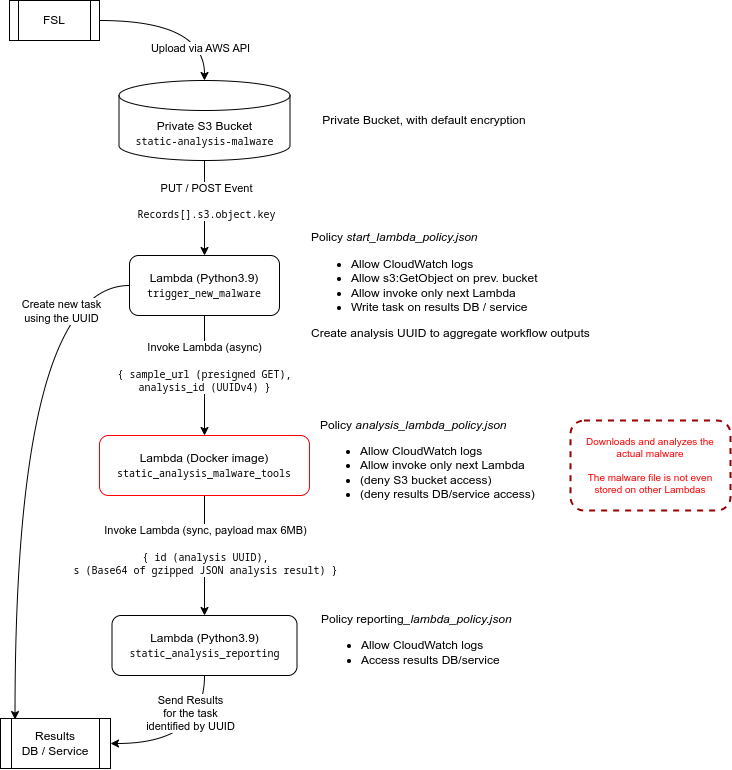
\includegraphics[width=\textwidth]{assets/aws_static_lambdas_architecture.png}
    \caption{Archittetura su AWS con i vari componenti coinvolti}
    \label{fig:aws_static_lambdas_architecture}
\end{figure}

\begin{figure}[htbp]
    \centering
    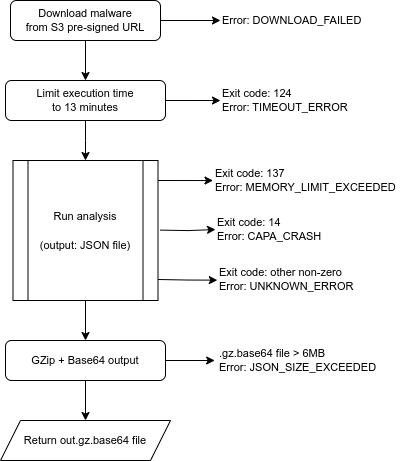
\includegraphics[width=0.75\textwidth]{assets/docker_static_analysis_flow.png}
    \caption{Workflow dell'analisi in \texttt{static\_analysis\_malware\_tools} e possibili errori}
    \label{fig:tools_workflow_static_analysis}
\end{figure}

All'interno della lambda di analisi viene aggiunto un nuovo script da usare come cmd (\texttt{lambda\_entrypoint.sh)}: ha lo scopo di fornire l'interfaccia runtime Lambda necessaria per l'esecuzione in tale runtime.
Non è possibile eseguire direttamente una immagine Docker così com'è su AWS Lambda, ma necessita di esporre una precisa interfaccia per compatibilità. Per rispettare questo requisito si può scegliere tra usare i container forniti da Amazon come base o usare altri strumenti. Nel nostro caso, trattandosi di un container molto poco straightforward, si è optati per la seconda opzione. È stato sufficiente invocare il modulo \texttt{awslambdaric} per eseguire uno script Python che espone una funzione avente la stessa interfaccia che ci si aspetta da una Lambda standard Python, ossia una funzione handler che accetti due parametri: l'evento e il context. Ci interessa principalmente l'evento, contenente il payload ricevuto durante l'invocazione.

Infine, per permettere anche un test della Lambda all'interno di una più simile runtime possibile all'ambiente di produzione, si sfrutta \texttt{aws-lambda-rie}, un tester con cui è possibile simulare l'ambiente finale eseguendo in locale.

\subsection{Limiti delle Lambda}
È bene sottolineare come le Lambda non siano lo strumento di computazione adatto in tutti i casi. In questa sezione vengono esposti i contro e le limitazioni che comportano, nonché i rimedi adottati per limitarne gli effetti.

Una delle prime limitazioni riguarda le risorse concesse dal server in termini di potenza di calcolo. Viene imposto a tutte le invocazioni un timeout estendibile fino a 15 minuti, e la potenza della CPU assegnata è proporzionale alla memoria richiesta.
È fondamentale essere consapevoli di tali caratteristiche del servizio, così da prendere contromisure quanto più efficiaci possibili.

Prima di tutto, si procede a misurare il tempo di esecuzione e la memoria richiesta da ogni analisi così da avere dei dati ottenuti da misurazioni su cui lavorare. Nell'immagine Docker precedentemente realizzata, si va ad eseguire il processo di analisi attraverso \texttt{/usr/bin/time}, da non confondere con il comando \texttt{time} generalmente integrato nella shell - sono distinguibili ed elencabili eseguendo il comando \texttt{type -a time}. L'eseguibile GNU, con il flag \texttt{-v}, permette di misurare sia il tempo di esecuzione che la memoria totale richiesta, consentendoci di eseguire delle stime. L'output verrà così salvato su un file testuale per poi essere analizzato, traendone più informazioni dai dati ottenuti.

Successivamente, eseguiamo il container così modificato su un sample set composto da 40 eseguibili scelti casualmente da VirusTotal, estraendo output e misurazioni. Infine, raccogliamo i dati in un grafico (figg. \ref{fig:static_analysis_exec_cpu_time} e \ref{fig:static_analysis_exec_memory}) per visualizzare il tempo e la memoria, tracciando una linea per rappresentare il valore medio. Notiamo come il tempo medio di esecuzione sia di circa 71 secondi, di gran lunga inferiore al limite di 15 minuti, ossia 900 secondi, per invocazione. Tuttavia, seppur non particolarmente grave, abbiamo appena citato come la potenza computazionale attesa sull'ambiente Lambda sia proporzionale alla memoria massima stabilita come allocabile e comunque inferiore a un ambiente di esecuzione locale riservato solo a questo scopo, per cui è da usare tali stime solo come un punto di riferimento vago, e non sottovalutare casi in cui questo possa aumentare fino a superare il timeout.
Proprio per ciò, viene imposto un limite già all'interno del container di esecuzione a 13 minuti per l'analisi, usando il comando \texttt{timeout} della shell, così da avere il tempo per permettere una situazione di \emph{graceful exit} e portare sempre a un output, che in questo caso conterrà il flag di successo a \texttt{false}, assieme al campo \texttt{"error"} valorizzato.

Per quanto concerne l'utilizzo di memoria, ci si attesta attorno ai 500MB circa di consumo, seppur non segua affatto una distribuzione normale, visto come ci siano sample che richiedano molta più memoria e altri molta meno, quasi nessuno quanto la media. Anche per questa casistica bisogna tenere conto dei casi di fallimento e prevedere una \emph{graceful exit}. Siccome si è visto che la quasi totalità dell'uso è dovuto dall'esecuzione di \texttt{capa}, si è voluto osservare il suo comportamento in caso di ragggiungimento del limite di memoria disponibile. Perciò, sfruttando il flag \texttt{--memory} di Docker run, si è impostato un limite molto basso e si osservano i risultati. Si è subito rilevato come ciò comportava un crash del tool specifico con exit code 137, associato proprio alla condizione di OOM (Out-Of-Memory). Il flusso di esecuzione però poteva continuare l'esecuzione, a patto di gestire l'errore, dovuto dal fatto che all'inizio dello script di analisi è stato impostato il flag \texttt{set -e} che comporta un'uscita automatica appena un comando dovesse restituire un exit code non-zero. La soluzione adottata è quella di gestire l'errore nello script chiamante, a livello più alto, quindi interrompendo l'analisi ma dando in output l'errore in maniera analoga a quanto indicato per il precedente caso del timeout.

Questa gestione degli errori porta il vantaggio di avere sempre in output un JSON valido, sempre presente e in grado di fornire un'indicazione dell'errore al processo invocante (nel caso finale sarà la Threat Intelligence prQuesta gestione degli errori porta il vantaggio di avere sempre in output un JSON valido, sempre presente e in grado di fornire un'indicazione dell'errore al processo invocante (nel caso finale sarà la Threat Intelligence presumibilmente).

\begin{figure}[htbp]
     \begin{subfigure}[b]{0.5\textwidth}
         \centering
         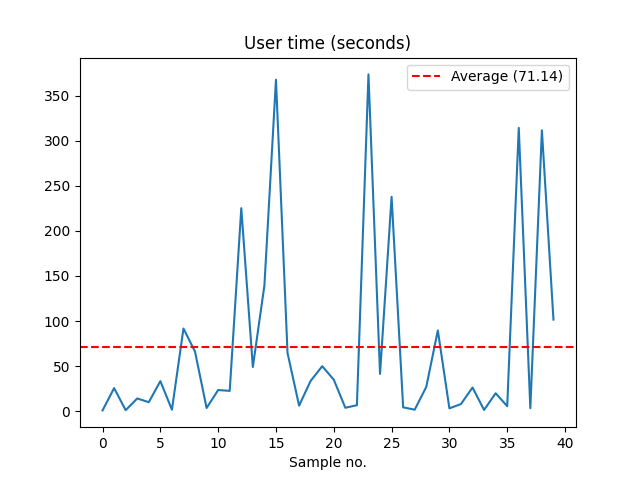
\includegraphics[width=\textwidth]{assets/static_analysis_exec_cpu_time.png}
         \caption{CPU}
         \label{fig:static_analysis_exec_cpu_time}
     \end{subfigure}
     \begin{subfigure}[b]{0.5\textwidth}
         \centering
         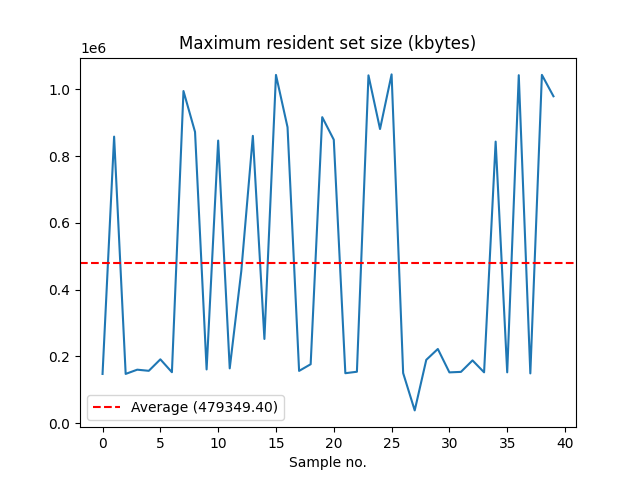
\includegraphics[width=\textwidth]{assets/static_analysis_exec_memory.png}
         \caption{Memoria}
         \label{fig:static_analysis_exec_memory}
     \end{subfigure}
     \caption{Uso delle risorse eseguendo analisi statica su malware reali presi a campione}
\end{figure}

Non si è ritenuto necessario procedere con l'upload dei risultati in un bucket S3, nè é ragionevole concedere alla Lambda di analisi il ruolo di contattare il sistema di reporting, che sia l'API della Threat Intelligence o un mock temporaneo, per i motivi di sicurezza precedentemente elencati. L'unica soluzione restante è quella di inviare il risultato come payload alla Lambda responsabile di quest'ultimo step. Tuttavia, AWS impone certi limiti per questa operazione: in caso di invocazione asincrona non può superare i 256KB, aumentabile fino a 6MB andando a usare l'invocazione sincrona. Quest'ultima ha lo svantaggio di addebitare il proprio tempo di esecuzione anche alla Lambda chiamante, ma non essendo un'operazione più lunga di pochissimi secondi, è un compromesso che si è disposti ad accettare.

Presa conoscienza di tale limite aggiuntivo, si procede ad effettuare una misurazione della dimensione in byte del JSON di output, già minimizzato e non formattato. Siccome è subito intuibile come questo possa essere troppo spesso oltre questa dimensione, si implementa una strategia per ridurne la dimensione.
Una prima idea poteva essere l'uso di una struttura \emph{"dizionari di liste"} al posto della più tradizionale \emph{"dizionari di liste"} comunemente adottata. Tuttavia, è stata scartata perché, seppur sarebbe andata a ridurre in maniera sensibile alcune strutture, come nel caso di liste con all'interno una lunga serie di dizionari, comportando l'inutile ripetizione delle stringhe delle chiavi dei dizionari interni, avrebbe comportato un'eccessiva trasformazione e molta meno flessibilità di modifica del formato o l'aggiunta/rimozioni di alcune sue parti.

La soluzione realmente adottata è stata usare \texttt{gzip}, un comune strumento di compressione che usa l'algoritmo \emph{DEFLATE}, usato con il massimo livello di aggressività,
per ridurre in maniera sostanziale lo spazio occupato dal JSON,
sfruttando le sue proprietà come l'essere un file testuale, avere spesso ripetizioni come nel caso delle chiavi dei dizionari e altre caratteristiche che ne favoriscono la comprimibilità.
Infine è necessario svolgere un ulteriore passaggio, visto che il payload delle Lambda non può essere uno stream di byte ma è richiesto che sia un oggetto JSON valido, quindi contenente testo. 
Viene preso il payload in byte ottenuto come risultato della compressione, e trasformato in testo adottando la codifica \emph{Base64} che però incrementa la dimensione di circa il 33\%, incluso in un JSON minimale avente solo la chiave \texttt{"s"} con all'interno questa codifica.

Dopo aver implementato questa strategia, è stata eseguita una misurazione paragonando la dimensione originale del JSON originale, del JSON codificato come appena illustrato e il livello dei 6MB come limite di ciò che è possibile inviare (fig. \ref{fig:static_analysis_results_size}). Si nota immediatamente come la dimensione della linea della versione codificata sia notevolmente inferiore a quella del file originale, abbattendo le probabilità di andare oltre il limite.
Siccome improbabile non significa impossibile, è stato d'obbligo prevedere una graceful exit anche in tale evenienza.

\begin{figure}[htbp]
    \centering
    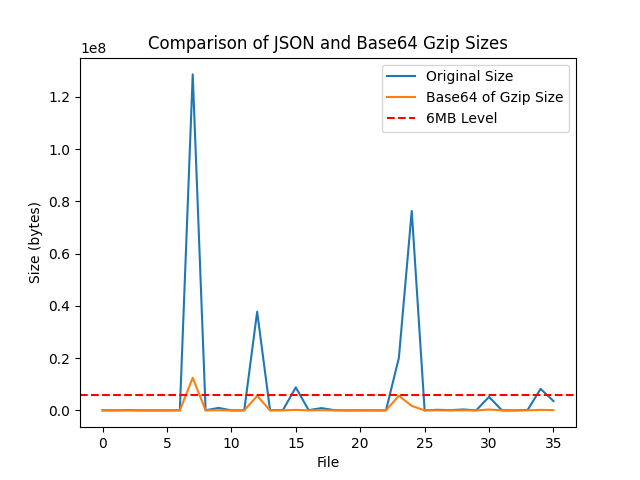
\includegraphics[width=0.6\textwidth]{assets/static_analysis_results_size.png}
    \caption{Dimensione del file di output originale e post-compressione gzip + base64}
    \label{fig:static_analysis_results_size}
\end{figure}

Per riassumere tutti i casi di errore evidenziati,
è stata definita e documentata una lista chiara dei codici di errore che possono verificarsi, ossia:
\begin{itemize}
    \item \texttt{TIMEOUT} per i casi di timeout, riconoscibili dall'exit code del comando timeout uguale a 124
    \item \texttt{MEMORY\_LIMIT\_EXCEEDED} attribuito all'exit code 137 (OOM) in caso di superamento del limite di memoria
    \item \texttt{DOWNLOAD\_FAILED} se nello script che accetta un URL come parametro e non direttamente, la richiesta HTTP è fallita sia per problemi di connessione che di status code della risposta non 2xx
    \item \texttt{CAPA\_CRASH\_UNKNOWN} assegnato al crash di capa, strumento più delicato di tutto il processo, diverso da motivazioni già precedentemente gestite
    \item \texttt{JSON\_SIZE\_EXCEEDED} nei casi di un output JSON riuscito con successo ma eccessivamente grande da superare i limiti di payload di invocazione delle Lambda
    \item \texttt{UNKNOWN\_ERROR} paragonabile a una risposta HTTP 500 Internal Server Error di un webserver, dove non è ben chiara la causa del crash ed è bene controllare i log
    \item \texttt{FATAL\_SCRIPT\_CRASH} nei casi più estremi in cui lo script di analisi non riesce a generare nè un successo nè un errore nel JSON di output, allora l'ultimo attore rimasto presente è l'handler Python della Lambda, che procederà ad emettere questo errore; si presuppone non succeda mai ma è conservato come ultimo tentativo di emettere un errore, in caso si verifichino situazioni molto più particolari non previste
\end{itemize}

La verifica che questi siano gli unici e i soli codici di errore restituibili in output è data dal sistema usato per creare il JSON di errore: uno script Python che da argomento da terminale prende in input l'errore che si vorrebbe restituire, controlla che sia tra quelli consentiti o ne restituisce uno di default segnalando l'avvenimento fuori dal protocollo definito nei log, per poi creare il JSON con il formato standard solo in caso non sia già stato dato un altro errore per la stessa invocazione. Quest'ultimo può essere rappresentato dal caso in cui la propagazione dell'exit code fallisca e la seconda volta venga richiesta l'emissione di un errore meno specifico, che lo script Python andrà a rifiutare.

\subsection{Costi del servizio}
Le prossime analisi si baseranno sui seguenti parametri di riferimento forniti sulla base dello storico aziendale e delle aspettative di uso reale del servizio:
\begin{table}[H]
    \centering
    \begin{tabular}{|l|l|}
        \hline
        \textbf{Parametro}             & \textbf{Valore}                 \\ \hline
        Numero di sample da analizzare & 100.000 al mese                 \\
        Memoria media richiesta        & 512 MB (limite massimo: 1024MB) \\
        Tempi medio di esecuzione      & 70 secondi                      \\ \hline
    \end{tabular}
\end{table}

Inoltre, si sottolinea come i costi dei servizi AWS subiscano inflessioni nel tempo, per cui questa stima è sufficientemente valida al momento della scrittura di questa relazione.
Per i calcoli viene usato il calcolatore ufficiale Amazon\footnote{\url{https://calculator.aws}}
inserendo come posizione Milano (eu-south-1) per ragioni di GDPR, policy aziendali e distanza dal server che effettuerà l'upload dei sample. In merito al numero di GET stimate al mese, si considerano, per ogni sample, 1 GET per la lettura nell'analisi e il 20\% delle volte una GET su Internet per il download del file dall'analista.
Viene escluso dai calcoli, l'uso del Free Tier, in quanto questo potrebbe essere utilizzato per ulteriori progetti sullo stesso account.

\begin{table}[H]
\centering
\begin{tabular}{|l|l|}
\hline
Dimensione media di un sample          & 1 MB                \\
Richieste PUT al mese                  & 100.000             \\
Richieste GET al mese                  & 120.000             \\
Numero di sample dopo 3 mesi           & 300.000             \\
Spazio occupato dai sample dopo 3 mesi & 300.000 MB $\approx$ 280 GB \\ \hline
Costo stimato mensile                  & € 10,00             \\ \hline
\end{tabular}
\label{tab:aws_s3_costs}
\caption{Parametri per il costo di un bucket S3}
\end{table}

\begin{table}[H]
\centering
\begin{tabular}{|ll|}
\hline
\multicolumn{2}{|c|}{\textbf{Lambda trigger post-upload}}                               \\ \hline
\multicolumn{1}{|l|}{Durata di esecuzione media}     & 2 secondi                        \\
\multicolumn{1}{|l|}{Memoria allocata}               & 256 MB                           \\
\multicolumn{1}{|l|}{Costo stimato mensile}          & € 1,00                           \\ \hline
\multicolumn{2}{|c|}{\textbf{Lambda analisi con strumenti}}                             \\ \hline
\multicolumn{1}{|l|}{Durata di esecuzione media}     & 70 secondi, limitato a 14 minuti \\
\multicolumn{1}{|l|}{Memoria allocata}               & 1024 MB                          \\
\multicolumn{1}{|l|}{Costo stimato mensile}          & € 124,00                         \\ \hline
\multicolumn{2}{|c|}{\textbf{Lambda reporting}}                                         \\ \hline
\multicolumn{1}{|l|}{Durata di esecuzione media}     & 5 secondi                        \\
\multicolumn{1}{|l|}{Memoria allocata}               & 512 MB                           \\
\multicolumn{1}{|l|}{Costo stimato mensile}          & € 5,00                           \\ \hline
\multicolumn{1}{|l|}{Invocazioni di tutte le Lambda} & 100.000 al mese per Lambda       \\ \hline
\end{tabular}
\label{tab:aws_lambdas_costs}
\caption{Parametri per il costo delle varie Lambda}
\end{table}

\begin{table}[H]
    \centering
    \begin{tabular}{|l|r|}
        \hline
        \textbf{Servizio}            & \textbf{Stima} \\ \hline
        S3 Bucket (standard tier)    & € 10,00        \\
        Lambda start                 & € 1,00         \\
        Lambda di analisi            & € 124,00       \\
        Lambda di fine rapporto      & € 5,00         \\ \hline
        Costo stimato totale al mese & € 140,00       \\ \hline
    \end{tabular}
    \label{tab:aws_summary_costs}
    \caption{Riepilogo dei costi stimati per i singoli servizi}
\end{table}

Viste le spese per task analoghi già sostenute dall'azienda, è ritenuto un valido preventivo, anche in ottica di futuro reale utilizzo del progetto all'interno del più vasto sistema.

Sono state tuttavia valutate anche altre opzioni, come l'uso di una o più istanze EC2 pre-allocate, con posto di fronte un load balancer, nel tentativo di ridurre i costi. Tuttavia, non è stato efficace ma controproducente, andando anche a perdere le qualità delle Lambda quali l'auto-scaling e il costo nullo in caso di non utilizzo.

\section{Versioning}
Per il versioning, è stato creato un repository Git sul server GitLab aziendale.

Per ogni modifica viene creato un commit, come è standard.

Tuttavia, ci sono alcuni aspetti dell'organizzazione che è rilevante sottolineare.

\subsection{Branch Naming Convention}
Per la gestione del repository,e in particolare i suoi branch, si seguono rigidamente queste convenzioni:
\begin{itemize}
    \item \texttt{main} è il branch principale dove deve essere presente solo codice finito e considerabile stabile a tutti gli effetti;
    \item \texttt{develop} è dove si tiene il codice che si considera usabile ma non ancora sufficientemente testato o pronto all'uso in produzioni così com'è - su questo branch infine è dove viene fatto il merge dei successivi branch più specifici;
    \item \texttt{feature/<feat-name>} è l'insieme di tutti i branch, originati da \emph{develop}, dove si lavora all'implementazione di una specifica funzione - ciò permette di mantenere il branch \emph{develop} funzionante, privo di funzioni non completamente realizzate, e diminuisce le interferenze tra chi sta lavorando sulla stessa codebase ma su funzioni distinte tra loro - e il prefisso \textbf{feature/} identifica chiaramente che si tratta di un branch dove si lavora solo ed esclusivamente su una sola funzionalità;
    \item \texttt{refactor/<ref-name>} invece rappresenta l'insieme dei branch dove si fa, con diversi gradi di complessità, refactoring del codice - ad esempio, nel progetto è stato realizzato un branch di refactoring per passare dall'uso di \texttt{os.path} al modulo Python \texttt{pathlib} per una maggiore usabilità
\end{itemize}

Infine, per un maggiore controllo, il merge dai branch secondari (\texttt{feature/} e \texttt{refactor}) vengono fatti attraverso l'uso di \emph{Merge Request} (o \emph{Pull Request}, a seconda che si usa la nomenclatura di GitLab o di GitHub).
In questo modo, è possibile interagire sul merge commentando o richiedendo revisioni di co-workers.

Non siamo ancora giunti al punto di rilasciare il progetto e attribuirgli una versione, ma in tal caso è ideale usare convenzioni standard come \emph{Semantic Versioning}
\footnote{\url{https://semver.org/lang/it/}}
, e usare tale stringa come \textbf{tag} sul repository Git.

\begin{figure}[h!]
    \centering
    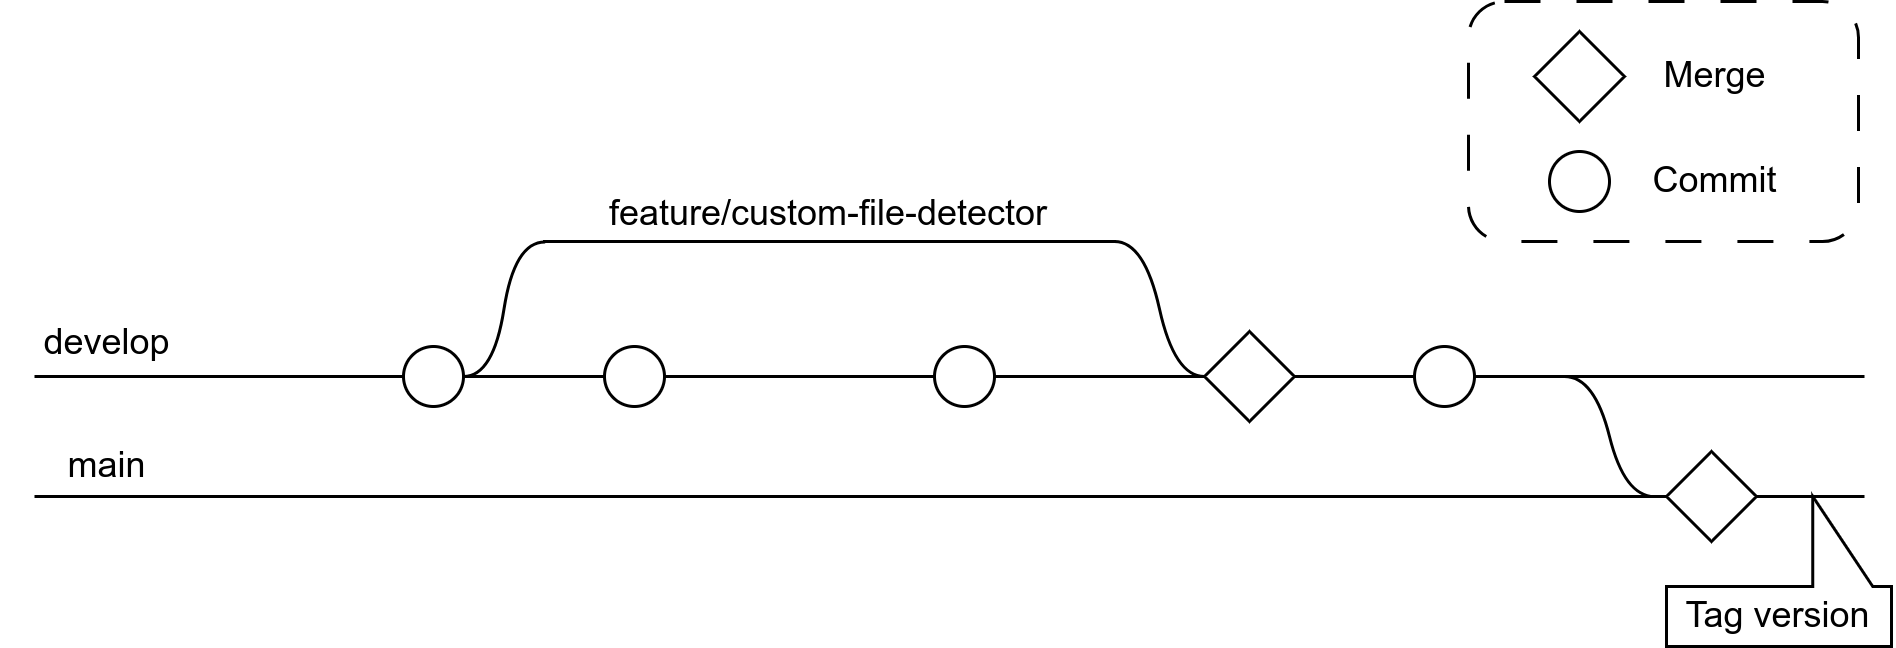
\includegraphics[width=\textwidth]{assets/git_branches_diagram.png}
    \caption{Struttura dei branch Git}
    \label{fig:git_branches_diagram}
\end{figure}

\section{CI/CD Pipeline}
Solo su develop = branch protetti
\chapter{Analisi dinamica}

\section{Cuckoo Sandbox}
Sandbox per fare le nostre analisi.
Come funziona?

\section{Multiscanner}
Strumento \cite{anacondacon_multiscanner}

Usiamo Cuckoo dentro Multiscanner per avere dei report migliori e future integrazioni con altri strumenti che Multiscanner offre.

\subsection{Hash fuzzing}
Sempre nella presentazione \cite{anacondacon_multiscanner} con \textbf{ssdeep} al minuto 16:00.

\chapter{Sviluppi futuri e integrazioni}

\section{Agger}

\subsection{EDR vs Antivirus}

\backmatter

\cleardoublepage
\phantomsection
\addcontentsline{toc}{chapter}{\bibname}
\bibliographystyle{sapthesis}
\bibliography{references}

\end{document}
